
\section{Calculating Exchanges}

\begin{enumerate}
\item Use Eq. $10.1$ to confirm Eq. $10.11$
\item Use Eq. $10.1$ to confirm Eq. $10.7$
\item Confirm the braiding relation $\hat{\sigma }_{1}\hat{\sigma }_{2}\hat{\sigma }_{1} =\hat{\sigma }_{2}\hat{\sigma }_{1}\hat{\sigma }_{2}$ in both cases. What does this identity mean geometrically. See exercise 3.1.
\end{enumerate}

\paragraph{Answer}

(a) Eq.10.1 is given by:
\begin{equation*}
\hat{\sigma }_{2} |c;f\rangle =\sum _{g,z} [F_{f}^{aaa} ]_{cg} R_{g}^{aa} [(F_{f}^{aaa} )^{-1} ]_{gz} |z;f\rangle .
\end{equation*}
For Ising anyons, the $F$ matrix is given by:
\begin{equation*}
F_{\sigma }^{\sigma \sigma \sigma } =\frac{1}{\sqrt{2}}\begin{pmatrix}
1 & 1\\
1 & -1
\end{pmatrix} =[F_{\sigma }^{\sigma \sigma \sigma } ]^{-1} ,
\end{equation*}
and the $R$ matrix is given by:
\begin{equation*}
\begin{aligned}
R_{I}^{\sigma \sigma } & =\mathrm{e}^{-\mathrm{i} \pi /8} ,\\
R_{\psi }^{\sigma \sigma } & =\mathrm{e}^{\mathrm{i} 3\pi /8} .
\end{aligned}
\end{equation*}
So we have directly
\begin{equation*}
\begin{aligned}
\hat{\sigma }_{2} |I;\sigma \rangle = & \sum _{g} ([F_{\sigma }^{\sigma \sigma \sigma } ]_{Ig} R_{g}^{\sigma \sigma } [(F_{\sigma }^{\sigma \sigma \sigma } )^{-1} ]_{gI} |I;\sigma \rangle +[F_{\sigma }^{\sigma \sigma \sigma } ]_{Ig} R_{g}^{\sigma \sigma } [(F_{\sigma }^{\sigma \sigma \sigma } )^{-1} ]_{g\psi } |\psi ;\sigma \rangle )\\
= & ([F_{\sigma }^{\sigma \sigma \sigma } ]_{II} R_{I}^{\sigma \sigma } [(F_{\sigma }^{\sigma \sigma \sigma } )^{-1} ]_{II} +[F_{\sigma }^{\sigma \sigma \sigma } ]_{I\psi } R_{\psi }^{\sigma \sigma } [(F_{\sigma }^{\sigma \sigma \sigma } )^{-1} ]_{\psi I} )|I;\sigma \rangle \\
+ & ([F_{\sigma }^{\sigma \sigma \sigma } ]_{II} R_{I}^{\sigma \sigma } [(F_{\sigma }^{\sigma \sigma \sigma } )^{-1} ]_{I\psi } +[F_{\sigma }^{\sigma \sigma \sigma } ]_{I\psi } R_{\psi }^{\sigma \sigma } [(F_{\sigma }^{\sigma \sigma \sigma } )^{-1} ]_{\psi \psi } )|\psi ;\sigma \rangle \\
= & \frac{1}{2} (\mathrm{e}^{-\mathrm{i} \pi /8} +\mathrm{e}^{\mathrm{i} 3\pi /8} )|I;\sigma \rangle +\frac{1}{2} (\mathrm{e}^{-\mathrm{i} \pi /3} -\mathrm{e}^{\mathrm{i} 3\pi /8} )|\psi ;\sigma \rangle \\
= & \frac{\mathrm{e}^{\mathrm{i} \pi /8}}{\sqrt{2}} (|I;\sigma \rangle -\mathrm{i} |\psi ;\sigma \rangle ).
\end{aligned}
\end{equation*}
For the second basis vector this is the same:
\begin{equation*}
\begin{aligned}
\hat{\sigma }_{2} |\psi ;\sigma \rangle  & =\sum _{g} ([F_{\sigma }^{\sigma \sigma \sigma } ]_{\psi g} R_{g}^{\sigma \sigma } [(F_{\sigma }^{\sigma \sigma \sigma } )^{-1} ]_{gI} |I;\sigma \rangle +[F_{\sigma }^{\sigma \sigma \sigma } ]_{\psi g} R_{g}^{\sigma \sigma } [(F_{\sigma }^{\sigma \sigma \sigma } )^{-1} ]_{g\psi } |\psi ;\sigma \rangle )\\
 & =\frac{\mathrm{e}^{\mathrm{i} \pi /8}}{\sqrt{2}} (-\mathrm{i} |I;\sigma \rangle +|\psi ;\sigma \rangle ).
\end{aligned}
\end{equation*}
Therefore, we have
\begin{equation*}
\hat{\sigma }_{2}\begin{pmatrix}
|I;\sigma \rangle \\
|\psi ;\sigma \rangle 
\end{pmatrix} =\frac{\mathrm{e}^{\mathrm{i} \pi /8}}{\sqrt{2}}\begin{pmatrix}
1 & -\mathrm{i}\\
-\mathrm{i} & 1
\end{pmatrix}\begin{pmatrix}
|I;\sigma \rangle \\
|\psi ;\sigma \rangle 
\end{pmatrix} ,
\end{equation*}
i.e.
\begin{equation*}
\hat{\sigma }_{2} =\frac{\mathrm{e}^{\mathrm{i} \pi /8}}{\sqrt{2}}\begin{pmatrix}
1 & -\mathrm{i}\\
-\mathrm{i} & 1
\end{pmatrix} .
\end{equation*}
(b) For Fibonacci Anyons, the non-trivial $F$ matrix is given by:
\begin{equation*}
F_{\tau }^{\tau \tau \tau } =\begin{pmatrix}
\phi ^{-1} & \phi ^{-1/2}\\
\phi ^{-1/2} & -\phi ^{-1}
\end{pmatrix} =[F_{\tau }^{\tau \tau \tau } ]^{-1} .
\end{equation*}
For $|0 \rangle =|I;\tau \rangle $, we have
\begin{equation*}
\begin{aligned}
\hat{\sigma }_{2} |0 \rangle = & (F_{00'} R_{I}^{\tau \tau } [F^{-1} ]_{0'0} +F_{01'} R_{\tau }^{\tau \tau } [F^{-1} ]_{10} )|0\rangle \\
+ & (F_{00'} R_{I}^{\tau \tau } [F^{-1} ]_{0'1} +F_{01'} R_{\tau }^{\tau \tau } [F^{-1} ]_{1'1} )|1\rangle \\
= & \phi ^{-1}\mathrm{e}^{4\pi \mathrm{i} /5} |0\rangle +\phi ^{-1/2}\mathrm{e}^{-3\pi \mathrm{i} /5} |1 \rangle ,
\end{aligned}
\end{equation*}
and for $|1 \rangle =|\tau ;\tau \rangle $, the procedure is the same:
\begin{equation*}
\hat{\sigma }_{2} |1\rangle =\phi ^{-1/2}\mathrm{e}^{-3\pi \mathrm{i} /5} |0 \rangle -\phi ^{-1} |1 \rangle .
\end{equation*}
For the single state $|N \rangle =|\tau ;I \rangle $, the $F$ matrix is just a number, which means
\begin{equation*}
\hat{\sigma }_{2} |N\rangle =R_{\tau }^{\tau \tau } |N\rangle =\mathrm{e}^{3\pi \mathrm{i} /5} .
\end{equation*}
Therefore, we have
\begin{equation*}
\hat{\sigma }_{2} =\begin{pmatrix}
\mathrm{e}^{3\pi \mathrm{i} /5} & 0 & 0\\
0 & \phi ^{-1}\mathrm{e}^{4\pi \mathrm{i} /5} & \phi ^{-1/2}\mathrm{e}^{-3\pi \mathrm{i} /5}\\
0 & \phi ^{-1/2}\mathrm{e}^{-3\pi \mathrm{i} /5} & -\phi ^{-1}
\end{pmatrix} .
\end{equation*}


(c) In first case:
\begin{equation*}
\hat{\sigma }_{1}\hat{\sigma }_{2}\hat{\sigma }_{1} =\frac{\mathrm{e}^{-\mathrm{i} \pi /8}}{\sqrt{2}}\begin{pmatrix}
1 & 1\\
1 & -1
\end{pmatrix} =\hat{\sigma }_{2}\hat{\sigma }_{1}\hat{\sigma }_{2} .
\end{equation*}
In the second case
\begin{equation*}
\hat{\sigma }_{1}\hat{\sigma }_{2}\hat{\sigma }_{1} =\begin{pmatrix}
\mathrm{e}^{-\pi \mathrm{i} /5} & 0 & 0\\
0 & -\phi \mathrm{^{-1} e}^{\pi \mathrm{i} /5} & \phi ^{-1/2} \phi ^{-4\mathrm{i} \pi /5}\\
0 & \phi ^{-1/2} \phi ^{-4\mathrm{i} \pi /5} & \phi ^{-1}\mathrm{e}^{\mathrm{i} \pi /5}
\end{pmatrix} =\hat{\sigma }_{2}\hat{\sigma }_{1}\hat{\sigma }_{2} .
\end{equation*}
Geometrically, this means the Yang-Baxter Equation.

\section{Ising Anyons Redux}
In exercise $3.3$ we introduced a representation for the exchange matrices for Ising anyons which, for three anyons, would be of the form
\begin{equation*}
\begin{aligned}
\hat{\sigma }_{1} & =\frac{\mathrm{e}^{\mathrm{i} \alpha }}{\sqrt{2}}( 1+\gamma _{1} \gamma _{2})\\
\hat{\sigma }_{2} & =\frac{\mathrm{e}^{\mathrm{i} \alpha }}{\sqrt{2}}( 1+\gamma _{2} \gamma _{3})
\end{aligned}
\end{equation*}
where the $\gamma $ 's are Majorana operators defined by
\begin{equation*}
\{\gamma _{i} ,\gamma _{j}\} \equiv \gamma _{i} \gamma _{j} +\gamma _{j} \gamma _{i} =2\delta _{ij}
\end{equation*}
with $\gamma _{i} =\gamma _{i}^{\dagger }$.

Show that the exchange matrices in Eq. $10.11$ are equivalent to this representation. How does one represent the $|0\rangle $ and $|1\rangle $ state of the Hilbert space in this language? The answer may not be unique.

\paragraph{Answer}
In this case, we first write
\begin{equation*}
\hat{\sigma }_{1} =\mathrm{e}^{-\mathrm{i} \pi /8}\begin{pmatrix}
1 & 0\\
0 & \mathrm{i}
\end{pmatrix} =\mathrm{e}^{\mathrm{i} \pi /8}\mathrm{e}^{-\mathrm{i} \pi /4}\begin{pmatrix}
1 & 0\\
0 & \mathrm{i}
\end{pmatrix} =\frac{\mathrm{e}^{\mathrm{i} \pi /8}}{\sqrt{2}}\begin{pmatrix}
1-\mathrm{i} & 0\\
0 & \mathrm{i} +1
\end{pmatrix} .
\end{equation*}
Then we have directly $\alpha =\pi /8$ and
\begin{equation*}
\gamma _{1} \gamma _{2} =\begin{pmatrix}
-\mathrm{i} & 0\\
0 & \mathrm{i}
\end{pmatrix} ,\quad \gamma _{2} \gamma _{3} =\begin{pmatrix}
0 & -\mathrm{i}\\
-\mathrm{i} & 0
\end{pmatrix} .
\end{equation*}
For example, if we take
\begin{equation*}
\gamma _{1} =\sigma _{1} =\begin{pmatrix}
0 & 1\\
1 & 0
\end{pmatrix} ,\quad \gamma _{2} =-\sigma _{2} =\begin{pmatrix}
0 & \mathrm{i}\\
-\mathrm{i} & 0
\end{pmatrix} ,\quad \gamma _{3} =\sigma _{3} =\begin{pmatrix}
1 & 0\\
0 & -1
\end{pmatrix} ,
\end{equation*}
we can the the result. In this case, the creation operator is
\begin{equation*}
c_{12}^{\dagger } =\frac{1}{2}( \gamma _{1} +\mathrm{i} \gamma _{2}) =\begin{pmatrix}
0 & 0\\
1 & 0
\end{pmatrix} ,
\end{equation*}
and we have:
\begin{equation*}
\begin{aligned}
c_{12}^{\dagger } |0 \rangle  & =|1 \rangle \\
c_{12}^{\dagger } |1 \rangle  & =0.
\end{aligned}
\end{equation*}

\section{Exchanging More Particles}

\begin{enumerate}
\item Consider a system of 4 identical Ising anyons. Use the $F$ - and $R$-matrices to calculate the braid matrices $\hat{\sigma }_{1} ,\hat{\sigma }_{2}$, and $\hat{\sigma }_{3}$. (You should be able to check your answer using the Majorana representation of exercise 3.3.)
\item (Harder) Consider a system of 4 identical Fibonacci anyons. Use the $F$ and $R$-matrices to calculate the braid matrices $\hat{\sigma }_{1} ,\hat{\sigma }_{2}$, and $\hat{\sigma }_{3}$.
\end{enumerate}

\paragraph{Answer}
(a) For four $\sigma $ anyons, we have two kinds of results: $I$ or $\psi $. Each type have two possibilities, for example we have $|0;\psi \rangle \equiv |I;\psi \rangle $ and $|1;\psi \rangle =|\psi ;\psi \rangle $, as the Fig.\ref{fig:FourIsing} shows.

\begin{figure}[h!]
\centering
\tikzset{every picture/.style={line width=0.75pt}} %set default line width to 0.75pt        

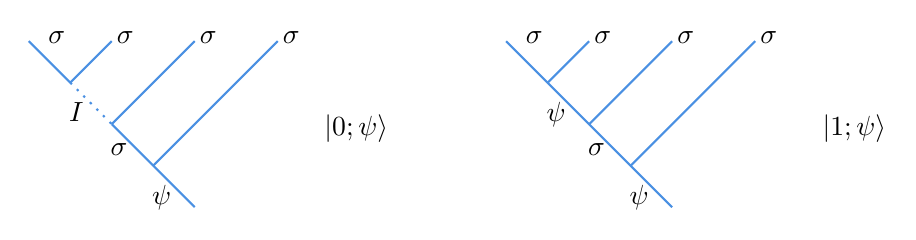
\begin{tikzpicture}[x=0.75pt,y=0.75pt,yscale=-1,xscale=1]
%uncomment if require: \path (0,98); %set diagram left start at 0, and has height of 98

%Straight Lines [id:da03295881017289837] 
\draw [color={rgb, 255:red, 74; green, 144; blue, 226 }  ,draw opacity=1 ]   (110,10) -- (130,30) ;
%Straight Lines [id:da934066087973815] 
\draw [color={rgb, 255:red, 74; green, 144; blue, 226 }  ,draw opacity=1 ]   (130,30) -- (150,10) ;
%Straight Lines [id:da6779658488228555] 
\draw [color={rgb, 255:red, 74; green, 144; blue, 226 }  ,draw opacity=1 ]   (150,50) -- (190,10) ;
%Straight Lines [id:da0783907422055814] 
\draw [color={rgb, 255:red, 74; green, 144; blue, 226 }  ,draw opacity=1 ]   (170,70) -- (230,10) ;
%Straight Lines [id:da9251509881333786] 
\draw [color={rgb, 255:red, 74; green, 144; blue, 226 }  ,draw opacity=1 ] [dash pattern={on 0.84pt off 2.51pt}]  (130,30) -- (150,50) ;
%Straight Lines [id:da6665710311354731] 
\draw [color={rgb, 255:red, 74; green, 144; blue, 226 }  ,draw opacity=1 ]   (150,50) -- (190,90) ;
%Straight Lines [id:da1366962949878192] 
\draw [color={rgb, 255:red, 74; green, 144; blue, 226 }  ,draw opacity=1 ]   (340,10) -- (420,90) ;
%Straight Lines [id:da740236469776278] 
\draw [color={rgb, 255:red, 74; green, 144; blue, 226 }  ,draw opacity=1 ]   (360,30) -- (380,10) ;
%Straight Lines [id:da04771683906239277] 
\draw [color={rgb, 255:red, 74; green, 144; blue, 226 }  ,draw opacity=1 ]   (380,50) -- (420,10) ;
%Straight Lines [id:da0532569568994119] 
\draw [color={rgb, 255:red, 74; green, 144; blue, 226 }  ,draw opacity=1 ]   (400,70) -- (460,10) ;

% Text Node
\draw (118,4) node [anchor=north west][inner sep=0.75pt]    {$\sigma $};
% Text Node
\draw (151,4) node [anchor=north west][inner sep=0.75pt]    {$\sigma $};
% Text Node
\draw (191,4) node [anchor=north west][inner sep=0.75pt]    {$\sigma $};
% Text Node
\draw (231,4) node [anchor=north west][inner sep=0.75pt]    {$\sigma $};
% Text Node
\draw (128,38) node [anchor=north west][inner sep=0.75pt]    {$I$};
% Text Node
\draw (148,58) node [anchor=north west][inner sep=0.75pt]    {$\sigma $};
% Text Node
\draw (168,78) node [anchor=north west][inner sep=0.75pt]    {$\psi $};
% Text Node
\draw (348,4) node [anchor=north west][inner sep=0.75pt]    {$\sigma $};
% Text Node
\draw (381,4) node [anchor=north west][inner sep=0.75pt]    {$\sigma $};
% Text Node
\draw (421,4) node [anchor=north west][inner sep=0.75pt]    {$\sigma $};
% Text Node
\draw (461,4) node [anchor=north west][inner sep=0.75pt]    {$\sigma $};
% Text Node
\draw (358,38) node [anchor=north west][inner sep=0.75pt]    {$\psi $};
% Text Node
\draw (378,58) node [anchor=north west][inner sep=0.75pt]    {$\sigma $};
% Text Node
\draw (398,78) node [anchor=north west][inner sep=0.75pt]    {$\psi $};
% Text Node
\draw (251,44) node [anchor=north west][inner sep=0.75pt]    {$|0;\psi \rangle $};
% Text Node
\draw (491,44) node [anchor=north west][inner sep=0.75pt]    {$|1;\psi \rangle $};
\end{tikzpicture}
\caption{Fusing channel of four identical Ising anyons.}
\label{fig:FourIsing}
\end{figure}

We just need to figure out the effect of $\hat{\sigma }_{3}$. Take $|0;\psi \rangle $ as example, we first change into basis that the third $\sigma $ and fourth $\sigma $ fuse first:
\begin{equation*}
\tikzset{every picture/.style={line width=0.75pt}} %set default line width to 0.75pt        
\begin{tikzpicture}[x=0.75pt,y=0.75pt,yscale=-1,xscale=1, baseline=(XXXX.south) ]
\path (0,91);\path (135.9777374267578,0);\draw    ($(current bounding box.center)+(0,0.3em)$) node [anchor=south] (XXXX) {};
%Straight Lines [id:da6082325711451675] 
\draw [color={rgb, 255:red, 74; green, 144; blue, 226 }  ,draw opacity=1 ]   (4,5) -- (24,25) ;
%Straight Lines [id:da6526565041271224] 
\draw [color={rgb, 255:red, 74; green, 144; blue, 226 }  ,draw opacity=1 ]   (24,25) -- (44,5) ;
%Straight Lines [id:da5438308378675105] 
\draw [color={rgb, 255:red, 74; green, 144; blue, 226 }  ,draw opacity=1 ]   (44,45) -- (84,5) ;
%Straight Lines [id:da46595828020710983] 
\draw [color={rgb, 255:red, 74; green, 144; blue, 226 }  ,draw opacity=1 ]   (64,65) -- (124,5) ;
%Straight Lines [id:da8660768427766763] 
\draw [color={rgb, 255:red, 74; green, 144; blue, 226 }  ,draw opacity=1 ] [dash pattern={on 0.84pt off 2.51pt}]  (24,25) -- (44,45) ;
%Straight Lines [id:da034969405295960376] 
\draw [color={rgb, 255:red, 74; green, 144; blue, 226 }  ,draw opacity=1 ]   (44,45) -- (84,85) ;
% Text Node
\draw (12,-2.5) node [anchor=north west][inner sep=0.75pt]    {$\sigma $};
% Text Node
\draw (45,-2.5) node [anchor=north west][inner sep=0.75pt]    {$\sigma $};
% Text Node
\draw (85,-2.5) node [anchor=north west][inner sep=0.75pt]    {$\sigma $};
% Text Node
\draw (125,-2.5) node [anchor=north west][inner sep=0.75pt]    {$\sigma $};
% Text Node
\draw (22,31.5) node [anchor=north west][inner sep=0.75pt]    {$I$};
% Text Node
\draw (42,51.5) node [anchor=north west][inner sep=0.75pt]    {$\sigma $};
% Text Node
\draw (62,71.5) node [anchor=north west][inner sep=0.75pt]    {$\psi $};
\end{tikzpicture}
=[F_{\sigma }^{I\sigma \sigma } ]_{\sigma \psi }\tikzset{every picture/.style={line width=0.75pt}} %set default line width to 0.75pt        
\begin{tikzpicture}[x=0.75pt,y=0.75pt,yscale=-1,xscale=1, baseline=(XXXX.south) ]
\path (0,91);\path (135.9777374267578,0);\draw    ($(current bounding box.center)+(0,0.3em)$) node [anchor=south] (XXXX) {};
%Straight Lines [id:da9791556643470056] 
\draw [color={rgb, 255:red, 74; green, 144; blue, 226 }  ,draw opacity=1 ]   (4,5) -- (24,25) ;
%Straight Lines [id:da7093233698616634] 
\draw [color={rgb, 255:red, 74; green, 144; blue, 226 }  ,draw opacity=1 ]   (24,25) -- (44,5) ;
%Straight Lines [id:da08046941256593554] 
\draw [color={rgb, 255:red, 74; green, 144; blue, 226 }  ,draw opacity=1 ]   (104.25,25.25) -- (84,5) ;
%Straight Lines [id:da2545237392909354] 
\draw [color={rgb, 255:red, 74; green, 144; blue, 226 }  ,draw opacity=1 ]   (64,65) -- (124,5) ;
%Straight Lines [id:da44844688823755474] 
\draw [color={rgb, 255:red, 74; green, 144; blue, 226 }  ,draw opacity=1 ] [dash pattern={on 0.84pt off 2.51pt}]  (24,25) -- (64,65) ;
%Straight Lines [id:da4755886440368011] 
\draw [color={rgb, 255:red, 74; green, 144; blue, 226 }  ,draw opacity=1 ]   (64,65) -- (84,85) ;
% Text Node
\draw (12,-2.5) node [anchor=north west][inner sep=0.75pt]    {$\sigma $};
% Text Node
\draw (45,-2.5) node [anchor=north west][inner sep=0.75pt]    {$\sigma $};
% Text Node
\draw (90,-2.5) node [anchor=north west][inner sep=0.75pt]    {$\sigma $};
% Text Node
\draw (125,-2.5) node [anchor=north west][inner sep=0.75pt]    {$\sigma $};
% Text Node
\draw (22,31.5) node [anchor=north west][inner sep=0.75pt]    {$I$};
% Text Node
\draw (93,30.5) node [anchor=north west][inner sep=0.75pt]    {$\psi $};
% Text Node
\draw (62,71.5) node [anchor=north west][inner sep=0.75pt]    {$\psi $};
\end{tikzpicture}
=\tikzset{every picture/.style={line width=0.75pt}} %set default line width to 0.75pt        
\begin{tikzpicture}[x=0.75pt,y=0.75pt,yscale=-1,xscale=1, baseline=(XXXX.south) ]
\path (0,91);\path (135.9777374267578,0);\draw    ($(current bounding box.center)+(0,0.3em)$) node [anchor=south] (XXXX) {};
%Straight Lines [id:da5655123388195396] 
\draw [color={rgb, 255:red, 74; green, 144; blue, 226 }  ,draw opacity=1 ]   (4,5) -- (24,25) ;
%Straight Lines [id:da5535768468202793] 
\draw [color={rgb, 255:red, 74; green, 144; blue, 226 }  ,draw opacity=1 ]   (24,25) -- (44,5) ;
%Straight Lines [id:da031755457318370484] 
\draw [color={rgb, 255:red, 74; green, 144; blue, 226 }  ,draw opacity=1 ]   (104.25,25.25) -- (84,5) ;
%Straight Lines [id:da2159015772977555] 
\draw [color={rgb, 255:red, 74; green, 144; blue, 226 }  ,draw opacity=1 ]   (64,65) -- (124,5) ;
%Straight Lines [id:da6349801560470765] 
\draw [color={rgb, 255:red, 74; green, 144; blue, 226 }  ,draw opacity=1 ] [dash pattern={on 0.84pt off 2.51pt}]  (24,25) -- (64,65) ;
%Straight Lines [id:da28281925510555905] 
\draw [color={rgb, 255:red, 74; green, 144; blue, 226 }  ,draw opacity=1 ]   (64,65) -- (84,85) ;
% Text Node
\draw (12,-2.5) node [anchor=north west][inner sep=0.75pt]    {$\sigma $};
% Text Node
\draw (45,-2.5) node [anchor=north west][inner sep=0.75pt]    {$\sigma $};
% Text Node
\draw (90,-2.5) node [anchor=north west][inner sep=0.75pt]    {$\sigma $};
% Text Node
\draw (125,-2.5) node [anchor=north west][inner sep=0.75pt]    {$\sigma $};
% Text Node
\draw (22,31.5) node [anchor=north west][inner sep=0.75pt]    {$I$};
% Text Node
\draw (93,30.5) node [anchor=north west][inner sep=0.75pt]    {$\psi $};
% Text Node
\draw (62,71.5) node [anchor=north west][inner sep=0.75pt]    {$\psi $};
\end{tikzpicture}
.
\end{equation*}
Then braiding gives
\begin{equation*}
\begin{aligned}
\hat{\sigma }_{3}\tikzset{every picture/.style={line width=0.75pt}} %set default line width to 0.75pt        
\begin{tikzpicture}[x=0.75pt,y=0.75pt,yscale=-1,xscale=1, baseline=(XXXX.south) ]
\path (0,91);\path (135.9777374267578,0);\draw    ($(current bounding box.center)+(0,0.3em)$) node [anchor=south] (XXXX) {};
%Straight Lines [id:da28096651380300175] 
\draw [color={rgb, 255:red, 74; green, 144; blue, 226 }  ,draw opacity=1 ]   (4,5) -- (24,25) ;
%Straight Lines [id:da3926255521758524] 
\draw [color={rgb, 255:red, 74; green, 144; blue, 226 }  ,draw opacity=1 ]   (24,25) -- (44,5) ;
%Straight Lines [id:da29292862563169675] 
\draw [color={rgb, 255:red, 74; green, 144; blue, 226 }  ,draw opacity=1 ]   (44,45) -- (84,5) ;
%Straight Lines [id:da25006466288038043] 
\draw [color={rgb, 255:red, 74; green, 144; blue, 226 }  ,draw opacity=1 ]   (64,65) -- (124,5) ;
%Straight Lines [id:da7782579426467391] 
\draw [color={rgb, 255:red, 74; green, 144; blue, 226 }  ,draw opacity=1 ] [dash pattern={on 0.84pt off 2.51pt}]  (24,25) -- (44,45) ;
%Straight Lines [id:da4411841592789685] 
\draw [color={rgb, 255:red, 74; green, 144; blue, 226 }  ,draw opacity=1 ]   (44,45) -- (84,85) ;
% Text Node
\draw (12,-2.5) node [anchor=north west][inner sep=0.75pt]    {$\sigma $};
% Text Node
\draw (45,-2.5) node [anchor=north west][inner sep=0.75pt]    {$\sigma $};
% Text Node
\draw (85,-2.5) node [anchor=north west][inner sep=0.75pt]    {$\sigma $};
% Text Node
\draw (125,-2.5) node [anchor=north west][inner sep=0.75pt]    {$\sigma $};
% Text Node
\draw (22,31.5) node [anchor=north west][inner sep=0.75pt]    {$I$};
% Text Node
\draw (42,51.5) node [anchor=north west][inner sep=0.75pt]    {$\sigma $};
% Text Node
\draw (62,71.5) node [anchor=north west][inner sep=0.75pt]    {$\psi $};
\end{tikzpicture}
 & =R_{\psi }^{\sigma \sigma }\tikzset{every picture/.style={line width=0.75pt}} %set default line width to 0.75pt        
\begin{tikzpicture}[x=0.75pt,y=0.75pt,yscale=-1,xscale=1, baseline=(XXXX.south) ]
\path (0,91);\path (135.9777374267578,0);\draw    ($(current bounding box.center)+(0,0.3em)$) node [anchor=south] (XXXX) {};
%Straight Lines [id:da8158106822790281] 
\draw [color={rgb, 255:red, 74; green, 144; blue, 226 }  ,draw opacity=1 ]   (4,5) -- (24,25) ;
%Straight Lines [id:da5955360680197377] 
\draw [color={rgb, 255:red, 74; green, 144; blue, 226 }  ,draw opacity=1 ]   (24,25) -- (44,5) ;
%Straight Lines [id:da449621943625496] 
\draw [color={rgb, 255:red, 74; green, 144; blue, 226 }  ,draw opacity=1 ]   (104.25,25.25) -- (84,5) ;
%Straight Lines [id:da38934356382209456] 
\draw [color={rgb, 255:red, 74; green, 144; blue, 226 }  ,draw opacity=1 ]   (64,65) -- (124,5) ;
%Straight Lines [id:da08006692155530826] 
\draw [color={rgb, 255:red, 74; green, 144; blue, 226 }  ,draw opacity=1 ] [dash pattern={on 0.84pt off 2.51pt}]  (24,25) -- (64,65) ;
%Straight Lines [id:da7054154590102928] 
\draw [color={rgb, 255:red, 74; green, 144; blue, 226 }  ,draw opacity=1 ]   (64,65) -- (84,85) ;
% Text Node
\draw (12,-2.5) node [anchor=north west][inner sep=0.75pt]    {$\sigma $};
% Text Node
\draw (45,-2.5) node [anchor=north west][inner sep=0.75pt]    {$\sigma $};
% Text Node
\draw (90,-2.5) node [anchor=north west][inner sep=0.75pt]    {$\sigma $};
% Text Node
\draw (125,-2.5) node [anchor=north west][inner sep=0.75pt]    {$\sigma $};
% Text Node
\draw (22,31.5) node [anchor=north west][inner sep=0.75pt]    {$I$};
% Text Node
\draw (93,30.5) node [anchor=north west][inner sep=0.75pt]    {$\psi $};
% Text Node
\draw (62,71.5) node [anchor=north west][inner sep=0.75pt]    {$\psi $};
\end{tikzpicture}
\\
 & =\mathrm{e}^{3\pi \mathrm{i} /8}\tikzset{every picture/.style={line width=0.75pt}} %set default line width to 0.75pt        
\begin{tikzpicture}[x=0.75pt,y=0.75pt,yscale=-1,xscale=1, baseline=(XXXX.south) ]
\path (0,91);\path (135.9777374267578,0);\draw    ($(current bounding box.center)+(0,0.3em)$) node [anchor=south] (XXXX) {};
%Straight Lines [id:da17960281445380932] 
\draw [color={rgb, 255:red, 74; green, 144; blue, 226 }  ,draw opacity=1 ]   (4,5) -- (24,25) ;
%Straight Lines [id:da21779170391406444] 
\draw [color={rgb, 255:red, 74; green, 144; blue, 226 }  ,draw opacity=1 ]   (24,25) -- (44,5) ;
%Straight Lines [id:da6630103231878421] 
\draw [color={rgb, 255:red, 74; green, 144; blue, 226 }  ,draw opacity=1 ]   (104.25,25.25) -- (84,5) ;
%Straight Lines [id:da33990511740276164] 
\draw [color={rgb, 255:red, 74; green, 144; blue, 226 }  ,draw opacity=1 ]   (64,65) -- (124,5) ;
%Straight Lines [id:da8485056345977848] 
\draw [color={rgb, 255:red, 74; green, 144; blue, 226 }  ,draw opacity=1 ] [dash pattern={on 0.84pt off 2.51pt}]  (24,25) -- (64,65) ;
%Straight Lines [id:da16695077929513302] 
\draw [color={rgb, 255:red, 74; green, 144; blue, 226 }  ,draw opacity=1 ]   (64,65) -- (84,85) ;
% Text Node
\draw (12,-2.5) node [anchor=north west][inner sep=0.75pt]    {$\sigma $};
% Text Node
\draw (45,-2.5) node [anchor=north west][inner sep=0.75pt]    {$\sigma $};
% Text Node
\draw (90,-2.5) node [anchor=north west][inner sep=0.75pt]    {$\sigma $};
% Text Node
\draw (125,-2.5) node [anchor=north west][inner sep=0.75pt]    {$\sigma $};
% Text Node
\draw (22,31.5) node [anchor=north west][inner sep=0.75pt]    {$I$};
% Text Node
\draw (93,30.5) node [anchor=north west][inner sep=0.75pt]    {$\psi $};
% Text Node
\draw (62,71.5) node [anchor=north west][inner sep=0.75pt]    {$\psi $};
\end{tikzpicture}
=\mathrm{e}^{3\pi \mathrm{i} /8}\tikzset{every picture/.style={line width=0.75pt}} %set default line width to 0.75pt        
\begin{tikzpicture}[x=0.75pt,y=0.75pt,yscale=-1,xscale=1, baseline=(XXXX.south) ]
\path (0,91);\path (135.9777374267578,0);\draw    ($(current bounding box.center)+(0,0.3em)$) node [anchor=south] (XXXX) {};
%Straight Lines [id:da8582566186147713] 
\draw [color={rgb, 255:red, 74; green, 144; blue, 226 }  ,draw opacity=1 ]   (4,5) -- (24,25) ;
%Straight Lines [id:da45279597367744784] 
\draw [color={rgb, 255:red, 74; green, 144; blue, 226 }  ,draw opacity=1 ]   (24,25) -- (44,5) ;
%Straight Lines [id:da19482429033915905] 
\draw [color={rgb, 255:red, 74; green, 144; blue, 226 }  ,draw opacity=1 ]   (44,45) -- (84,5) ;
%Straight Lines [id:da08037142017831855] 
\draw [color={rgb, 255:red, 74; green, 144; blue, 226 }  ,draw opacity=1 ]   (64,65) -- (124,5) ;
%Straight Lines [id:da9868734897183242] 
\draw [color={rgb, 255:red, 74; green, 144; blue, 226 }  ,draw opacity=1 ] [dash pattern={on 0.84pt off 2.51pt}]  (24,25) -- (44,45) ;
%Straight Lines [id:da47608430023018466] 
\draw [color={rgb, 255:red, 74; green, 144; blue, 226 }  ,draw opacity=1 ]   (44,45) -- (84,85) ;
% Text Node
\draw (12,-2.5) node [anchor=north west][inner sep=0.75pt]    {$\sigma $};
% Text Node
\draw (45,-2.5) node [anchor=north west][inner sep=0.75pt]    {$\sigma $};
% Text Node
\draw (85,-2.5) node [anchor=north west][inner sep=0.75pt]    {$\sigma $};
% Text Node
\draw (125,-2.5) node [anchor=north west][inner sep=0.75pt]    {$\sigma $};
% Text Node
\draw (22,31.5) node [anchor=north west][inner sep=0.75pt]    {$I$};
% Text Node
\draw (42,51.5) node [anchor=north west][inner sep=0.75pt]    {$\sigma $};
% Text Node
\draw (62,71.5) node [anchor=north west][inner sep=0.75pt]    {$\psi $};
\end{tikzpicture}
.
\end{aligned}
\end{equation*}
For the second case:
\begin{equation*}
\tikzset{every picture/.style={line width=0.75pt}} %set default line width to 0.75pt        
\begin{tikzpicture}[x=0.75pt,y=0.75pt,yscale=-1,xscale=1, baseline=(XXXX.south) ]
\path (0,91);\path (135.9777374267578,0);\draw    ($(current bounding box.center)+(0,0.3em)$) node [anchor=south] (XXXX) {};
%Straight Lines [id:da7917556907528667] 
\draw [color={rgb, 255:red, 74; green, 144; blue, 226 }  ,draw opacity=1 ]   (2.98,6.97) -- (82.98,86.97) ;
%Straight Lines [id:da22814190573066817] 
\draw [color={rgb, 255:red, 74; green, 144; blue, 226 }  ,draw opacity=1 ]   (22.98,26.97) -- (42.98,6.97) ;
%Straight Lines [id:da387698957506071] 
\draw [color={rgb, 255:red, 74; green, 144; blue, 226 }  ,draw opacity=1 ]   (42.98,46.97) -- (82.98,6.97) ;
%Straight Lines [id:da7265065763418079] 
\draw [color={rgb, 255:red, 74; green, 144; blue, 226 }  ,draw opacity=1 ]   (62.98,66.97) -- (122.98,6.97) ;
% Text Node
\draw (10.98,-0.53) node [anchor=north west][inner sep=0.75pt]    {$\sigma $};
% Text Node
\draw (43.98,-0.53) node [anchor=north west][inner sep=0.75pt]    {$\sigma $};
% Text Node
\draw (83.98,-0.53) node [anchor=north west][inner sep=0.75pt]    {$\sigma $};
% Text Node
\draw (123.98,-0.53) node [anchor=north west][inner sep=0.75pt]    {$\sigma $};
% Text Node
\draw (20.98,33.47) node [anchor=north west][inner sep=0.75pt]    {$\psi $};
% Text Node
\draw (40.98,53.47) node [anchor=north west][inner sep=0.75pt]    {$\sigma $};
% Text Node
\draw (60.98,73.47) node [anchor=north west][inner sep=0.75pt]    {$\psi $};
\end{tikzpicture}
=[F_{\psi }^{\psi \sigma \sigma } ]_{\sigma I}\tikzset{every picture/.style={line width=0.75pt}} %set default line width to 0.75pt        
\begin{tikzpicture}[x=0.75pt,y=0.75pt,yscale=-1,xscale=1, baseline=(XXXX.south) ]
\path (0,91);\path (135.9777374267578,0);\draw    ($(current bounding box.center)+(0,0.3em)$) node [anchor=south] (XXXX) {};
%Straight Lines [id:da7736135833134192] 
\draw [color={rgb, 255:red, 74; green, 144; blue, 226 }  ,draw opacity=1 ]   (2.98,6.97) -- (82.98,86.97) ;
%Straight Lines [id:da33403757050720917] 
\draw [color={rgb, 255:red, 74; green, 144; blue, 226 }  ,draw opacity=1 ]   (22.98,26.97) -- (42.98,6.97) ;
%Straight Lines [id:da3837650947804325] 
\draw [color={rgb, 255:red, 74; green, 144; blue, 226 }  ,draw opacity=1 ]   (102.61,26.6) -- (82.98,6.97) ;
%Straight Lines [id:da49231520747222235] 
\draw [color={rgb, 255:red, 74; green, 144; blue, 226 }  ,draw opacity=1 ]   (102.61,26.6) -- (122.98,6.97) ;
%Straight Lines [id:da8244101167253088] 
\draw [color={rgb, 255:red, 74; green, 144; blue, 226 }  ,draw opacity=1 ] [dash pattern={on 0.84pt off 2.51pt}]  (62.98,66.97) -- (102.61,26.6) ;
% Text Node
\draw (10.98,-0.53) node [anchor=north west][inner sep=0.75pt]    {$\sigma $};
% Text Node
\draw (43.98,-0.53) node [anchor=north west][inner sep=0.75pt]    {$\sigma $};
% Text Node
\draw (89.98,-0.53) node [anchor=north west][inner sep=0.75pt]    {$\sigma $};
% Text Node
\draw (123.98,-0.53) node [anchor=north west][inner sep=0.75pt]    {$\sigma $};
% Text Node
\draw (20.98,33.47) node [anchor=north west][inner sep=0.75pt]    {$\psi $};
% Text Node
\draw (91.98,33.47) node [anchor=north west][inner sep=0.75pt]    {$I$};
% Text Node
\draw (60.98,73.47) node [anchor=north west][inner sep=0.75pt]    {$\psi $};
\end{tikzpicture}
,
\end{equation*}
Then braiding gives
\begin{equation*}
\begin{aligned}
\hat{\sigma }_{3}\tikzset{every picture/.style={line width=0.75pt}} %set default line width to 0.75pt        
\begin{tikzpicture}[x=0.75pt,y=0.75pt,yscale=-1,xscale=1, baseline=(XXXX.south) ]
\path (0,91);\path (135.9777374267578,0);\draw    ($(current bounding box.center)+(0,0.3em)$) node [anchor=south] (XXXX) {};
%Straight Lines [id:da9993575333573745] 
\draw [color={rgb, 255:red, 74; green, 144; blue, 226 }  ,draw opacity=1 ]   (2.98,6.97) -- (82.98,86.97) ;
%Straight Lines [id:da8659093852240587] 
\draw [color={rgb, 255:red, 74; green, 144; blue, 226 }  ,draw opacity=1 ]   (22.98,26.97) -- (42.98,6.97) ;
%Straight Lines [id:da5902721534473272] 
\draw [color={rgb, 255:red, 74; green, 144; blue, 226 }  ,draw opacity=1 ]   (42.98,46.97) -- (82.98,6.97) ;
%Straight Lines [id:da49853088948238655] 
\draw [color={rgb, 255:red, 74; green, 144; blue, 226 }  ,draw opacity=1 ]   (62.98,66.97) -- (122.98,6.97) ;
% Text Node
\draw (10.98,-0.53) node [anchor=north west][inner sep=0.75pt]    {$\sigma $};
% Text Node
\draw (43.98,-0.53) node [anchor=north west][inner sep=0.75pt]    {$\sigma $};
% Text Node
\draw (83.98,-0.53) node [anchor=north west][inner sep=0.75pt]    {$\sigma $};
% Text Node
\draw (123.98,-0.53) node [anchor=north west][inner sep=0.75pt]    {$\sigma $};
% Text Node
\draw (20.98,33.47) node [anchor=north west][inner sep=0.75pt]    {$\psi $};
% Text Node
\draw (40.98,53.47) node [anchor=north west][inner sep=0.75pt]    {$\sigma $};
% Text Node
\draw (60.98,73.47) node [anchor=north west][inner sep=0.75pt]    {$\psi $};
\end{tikzpicture}
 & =[F_{\psi }^{\psi \sigma \sigma } ]_{\sigma I} R_{I}^{\sigma \sigma }\tikzset{every picture/.style={line width=0.75pt}} %set default line width to 0.75pt        
\begin{tikzpicture}[x=0.75pt,y=0.75pt,yscale=-1,xscale=1, baseline=(XXXX.south) ]
\path (0,91);\path (135.9777374267578,0);\draw    ($(current bounding box.center)+(0,0.3em)$) node [anchor=south] (XXXX) {};
%Straight Lines [id:da4207807765507652] 
\draw [color={rgb, 255:red, 74; green, 144; blue, 226 }  ,draw opacity=1 ]   (2.98,6.97) -- (82.98,86.97) ;
%Straight Lines [id:da03361530341663643] 
\draw [color={rgb, 255:red, 74; green, 144; blue, 226 }  ,draw opacity=1 ]   (22.98,26.97) -- (42.98,6.97) ;
%Straight Lines [id:da08014279215291031] 
\draw [color={rgb, 255:red, 74; green, 144; blue, 226 }  ,draw opacity=1 ]   (102.61,26.6) -- (82.98,6.97) ;
%Straight Lines [id:da11470234452659023] 
\draw [color={rgb, 255:red, 74; green, 144; blue, 226 }  ,draw opacity=1 ]   (102.61,26.6) -- (122.98,6.97) ;
%Straight Lines [id:da8447139048479473] 
\draw [color={rgb, 255:red, 74; green, 144; blue, 226 }  ,draw opacity=1 ] [dash pattern={on 0.84pt off 2.51pt}]  (62.98,66.97) -- (102.61,26.6) ;
% Text Node
\draw (10.98,-0.53) node [anchor=north west][inner sep=0.75pt]    {$\sigma $};
% Text Node
\draw (43.98,-0.53) node [anchor=north west][inner sep=0.75pt]    {$\sigma $};
% Text Node
\draw (89.98,-0.53) node [anchor=north west][inner sep=0.75pt]    {$\sigma $};
% Text Node
\draw (123.98,-0.53) node [anchor=north west][inner sep=0.75pt]    {$\sigma $};
% Text Node
\draw (20.98,33.47) node [anchor=north west][inner sep=0.75pt]    {$\psi $};
% Text Node
\draw (91.98,33.47) node [anchor=north west][inner sep=0.75pt]    {$I$};
% Text Node
\draw (60.98,73.47) node [anchor=north west][inner sep=0.75pt]    {$\psi $};
\end{tikzpicture}
\\
 & =\mathrm{e}^{-\mathrm{i} \pi /8}\tikzset{every picture/.style={line width=0.75pt}} %set default line width to 0.75pt        
\begin{tikzpicture}[x=0.75pt,y=0.75pt,yscale=-1,xscale=1, baseline=(XXXX.south) ]
\path (0,91);\path (135.9777374267578,0);\draw    ($(current bounding box.center)+(0,0.3em)$) node [anchor=south] (XXXX) {};
%Straight Lines [id:da9327048295091567] 
\draw [color={rgb, 255:red, 74; green, 144; blue, 226 }  ,draw opacity=1 ]   (2.98,6.97) -- (82.98,86.97) ;
%Straight Lines [id:da8973619839396276] 
\draw [color={rgb, 255:red, 74; green, 144; blue, 226 }  ,draw opacity=1 ]   (22.98,26.97) -- (42.98,6.97) ;
%Straight Lines [id:da14585819010027312] 
\draw [color={rgb, 255:red, 74; green, 144; blue, 226 }  ,draw opacity=1 ]   (42.98,46.97) -- (82.98,6.97) ;
%Straight Lines [id:da24040377018545223] 
\draw [color={rgb, 255:red, 74; green, 144; blue, 226 }  ,draw opacity=1 ]   (62.98,66.97) -- (122.98,6.97) ;
% Text Node
\draw (10.98,-0.53) node [anchor=north west][inner sep=0.75pt]    {$\sigma $};
% Text Node
\draw (43.98,-0.53) node [anchor=north west][inner sep=0.75pt]    {$\sigma $};
% Text Node
\draw (83.98,-0.53) node [anchor=north west][inner sep=0.75pt]    {$\sigma $};
% Text Node
\draw (123.98,-0.53) node [anchor=north west][inner sep=0.75pt]    {$\sigma $};
% Text Node
\draw (20.98,33.47) node [anchor=north west][inner sep=0.75pt]    {$\psi $};
% Text Node
\draw (40.98,53.47) node [anchor=north west][inner sep=0.75pt]    {$\sigma $};
% Text Node
\draw (60.98,73.47) node [anchor=north west][inner sep=0.75pt]    {$\psi $};
\end{tikzpicture}
.
\end{aligned}
\end{equation*}
This means we have
\begin{equation*}
\hat{\sigma }_{3}\begin{pmatrix}
|0;\psi \rangle \\
|1;\psi \rangle 
\end{pmatrix} =\begin{pmatrix}
\mathrm{e}^{3\pi \mathrm{i} /8} |0;\psi \rangle \\
\mathrm{e}^{-\mathrm{i} \pi /8} |1;\psi \rangle 
\end{pmatrix} ,
\end{equation*}
i.e.
\begin{equation*}
\hat{\sigma }_{3} =\begin{pmatrix}
\mathrm{e}^{3\pi \mathrm{i} /8} & 0\\
0 & \mathrm{e}^{-\mathrm{i} \pi /8}
\end{pmatrix} .
\end{equation*}
If we try $|0;I \rangle ,|1;I \rangle $, we will get the same result. In Majorana representation, we can see
\begin{equation*}
\hat{\sigma }_{3} =\frac{\mathrm{e}^{\mathrm{i} \pi /8}}{\sqrt{2}}\begin{pmatrix}
1+\mathrm{i} & 0\\
0 & 1-\mathrm{i}
\end{pmatrix} =\frac{\mathrm{e}^{\mathrm{i} \pi /8}}{\sqrt{2}}( 1+\gamma _{3} \gamma _{4}) ,
\end{equation*}
with $\gamma _{3} =\sigma _{3}$, we have
\begin{equation*}
\gamma _{4} =\begin{pmatrix}
\mathrm{i} & \\
 & \mathrm{i}
\end{pmatrix} ,
\end{equation*}
which satisfies the condition $\{\gamma _{i} ,\gamma _{j}\} =2\delta _{ij}$. So for the full space,in the order $|0;I \rangle ,|1;I \rangle ,|0;\psi \rangle ,|1;\psi \rangle $, we have
\begin{equation*}
\hat{\sigma }_{1,\text{full}} =\begin{pmatrix}
\hat{\sigma }_{1} & \\
 & \hat{\sigma }_{1}
\end{pmatrix} ,\quad \hat{\sigma }_{2,\text{full}} =\begin{pmatrix}
\hat{\sigma }_{2} & \\
 & \hat{\sigma }_{2}
\end{pmatrix} ,\quad \hat{\sigma }_{3,\text{full}} =\begin{pmatrix}
\hat{\sigma }_{3} & \\
 & \hat{\sigma }_{3}
\end{pmatrix} .
\end{equation*}

(b) With four $\tau $, we have $5$ possibilities, as the Fig.\ref{fig:FourFibonacci}  shows. 
\begin{figure}[h!]
\centering
\tikzset{every picture/.style={line width=0.75pt}} %set default line width to 0.75pt        

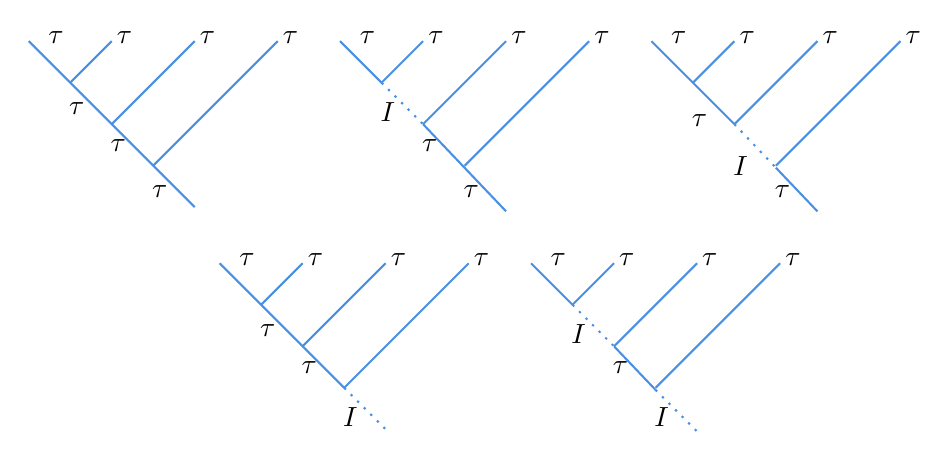
\begin{tikzpicture}[x=0.75pt,y=0.75pt,yscale=-1,xscale=1]
%uncomment if require: \path (0,204); %set diagram left start at 0, and has height of 204

%Straight Lines [id:da27255774977803204] 
\draw [color={rgb, 255:red, 74; green, 144; blue, 226 }  ,draw opacity=1 ]   (114,11) -- (194,91) ;
%Straight Lines [id:da9834488719668879] 
\draw [color={rgb, 255:red, 74; green, 144; blue, 226 }  ,draw opacity=1 ]   (134,31) -- (154,11) ;
%Straight Lines [id:da05252417338386017] 
\draw [color={rgb, 255:red, 74; green, 144; blue, 226 }  ,draw opacity=1 ]   (154,51) -- (194,11) ;
%Straight Lines [id:da03808367208482277] 
\draw [color={rgb, 255:red, 74; green, 144; blue, 226 }  ,draw opacity=1 ]   (174,71) -- (234,11) ;

%Straight Lines [id:da39898918953496443] 
\draw [color={rgb, 255:red, 74; green, 144; blue, 226 }  ,draw opacity=1 ]   (264,11) -- (284,31) ;
%Straight Lines [id:da19117790440950455] 
\draw [color={rgb, 255:red, 74; green, 144; blue, 226 }  ,draw opacity=1 ]   (284,31) -- (304,11) ;
%Straight Lines [id:da8810113330199636] 
\draw [color={rgb, 255:red, 74; green, 144; blue, 226 }  ,draw opacity=1 ]   (304,51) -- (344,11) ;
%Straight Lines [id:da4891521540730983] 
\draw [color={rgb, 255:red, 74; green, 144; blue, 226 }  ,draw opacity=1 ]   (324,71) -- (384,11) ;
%Straight Lines [id:da0036793482750658857] 
\draw [color={rgb, 255:red, 74; green, 144; blue, 226 }  ,draw opacity=1 ] [dash pattern={on 0.84pt off 2.51pt}]  (284,31) -- (304,51) ;
%Straight Lines [id:da16142694121534018] 
\draw [color={rgb, 255:red, 74; green, 144; blue, 226 }  ,draw opacity=1 ]   (304,51) -- (344,93) ;

%Straight Lines [id:da0588493597344828] 
\draw [color={rgb, 255:red, 74; green, 144; blue, 226 }  ,draw opacity=1 ]   (414,11) -- (434,31) ;
%Straight Lines [id:da46058436609013964] 
\draw [color={rgb, 255:red, 74; green, 144; blue, 226 }  ,draw opacity=1 ]   (434,31) -- (454,11) ;
%Straight Lines [id:da6535378534870788] 
\draw [color={rgb, 255:red, 74; green, 144; blue, 226 }  ,draw opacity=1 ]   (454,51) -- (494,11) ;
%Straight Lines [id:da9382789296032561] 
\draw [color={rgb, 255:red, 74; green, 144; blue, 226 }  ,draw opacity=1 ]   (474,71) -- (534,11) ;
%Straight Lines [id:da15832144021014827] 
\draw [color={rgb, 255:red, 74; green, 144; blue, 226 }  ,draw opacity=1 ] [dash pattern={on 0.84pt off 2.51pt}]  (454,51) -- (474,72) ;
%Straight Lines [id:da27626390664519684] 
\draw [color={rgb, 255:red, 74; green, 144; blue, 226 }  ,draw opacity=1 ]   (474,72) -- (494,93) ;
%Straight Lines [id:da7089065142284416] 
\draw [color={rgb, 255:red, 74; green, 144; blue, 226 }  ,draw opacity=1 ]   (434,31) -- (454,51) ;

%Straight Lines [id:da1997613978795223] 
\draw [color={rgb, 255:red, 74; green, 144; blue, 226 }  ,draw opacity=1 ]   (206,118) -- (266,178) ;
%Straight Lines [id:da11086690523449083] 
\draw [color={rgb, 255:red, 74; green, 144; blue, 226 }  ,draw opacity=1 ]   (226,138) -- (246,118) ;
%Straight Lines [id:da5779353066788016] 
\draw [color={rgb, 255:red, 74; green, 144; blue, 226 }  ,draw opacity=1 ]   (246,158) -- (286,118) ;
%Straight Lines [id:da5768885743980878] 
\draw [color={rgb, 255:red, 74; green, 144; blue, 226 }  ,draw opacity=1 ]   (266,178) -- (326,118) ;
%Straight Lines [id:da47066288819807567] 
\draw [color={rgb, 255:red, 74; green, 144; blue, 226 }  ,draw opacity=1 ] [dash pattern={on 0.84pt off 2.51pt}]  (266,178) -- (286,198) ;

%Straight Lines [id:da2811600003232293] 
\draw [color={rgb, 255:red, 74; green, 144; blue, 226 }  ,draw opacity=1 ]   (356,118) -- (376,138) ;
%Straight Lines [id:da7073679953842329] 
\draw [color={rgb, 255:red, 74; green, 144; blue, 226 }  ,draw opacity=1 ]   (376,138) -- (396,118) ;
%Straight Lines [id:da6328233857289285] 
\draw [color={rgb, 255:red, 74; green, 144; blue, 226 }  ,draw opacity=1 ]   (396,158) -- (436,118) ;
%Straight Lines [id:da5668048290766852] 
\draw [color={rgb, 255:red, 74; green, 144; blue, 226 }  ,draw opacity=1 ]   (416,178) -- (476,118) ;
%Straight Lines [id:da6525080893488078] 
\draw [color={rgb, 255:red, 74; green, 144; blue, 226 }  ,draw opacity=1 ] [dash pattern={on 0.84pt off 2.51pt}]  (376,138) -- (396,158) ;
%Straight Lines [id:da09143246778853076] 
\draw [color={rgb, 255:red, 74; green, 144; blue, 226 }  ,draw opacity=1 ]   (396,158) -- (416,179) ;
%Straight Lines [id:da03120788541808528] 
\draw [color={rgb, 255:red, 74; green, 144; blue, 226 }  ,draw opacity=1 ] [dash pattern={on 0.84pt off 2.51pt}]  (416,179) -- (436,199) ;


% Text Node
\draw (122,5) node [anchor=north west][inner sep=0.75pt]    {$\tau $};
% Text Node
\draw (155,5) node [anchor=north west][inner sep=0.75pt]    {$\tau $};
% Text Node
\draw (195,5) node [anchor=north west][inner sep=0.75pt]    {$\tau $};
% Text Node
\draw (235,5) node [anchor=north west][inner sep=0.75pt]    {$\tau $};
% Text Node
\draw (132,39) node [anchor=north west][inner sep=0.75pt]    {$\tau $};
% Text Node
\draw (152,57) node [anchor=north west][inner sep=0.75pt]    {$\tau $};
% Text Node
\draw (172,79) node [anchor=north west][inner sep=0.75pt]    {$\tau $};
% Text Node
\draw (272,5) node [anchor=north west][inner sep=0.75pt]    {$\tau $};
% Text Node
\draw (305,5) node [anchor=north west][inner sep=0.75pt]    {$\tau $};
% Text Node
\draw (345,5) node [anchor=north west][inner sep=0.75pt]    {$\tau $};
% Text Node
\draw (385,5) node [anchor=north west][inner sep=0.75pt]    {$\tau $};
% Text Node
\draw (282,39) node [anchor=north west][inner sep=0.75pt]    {$I$};
% Text Node
\draw (302,57) node [anchor=north west][inner sep=0.75pt]    {$\tau $};
% Text Node
\draw (322,79) node [anchor=north west][inner sep=0.75pt]    {$\tau $};
% Text Node
\draw (422,5) node [anchor=north west][inner sep=0.75pt]    {$\tau $};
% Text Node
\draw (455,5) node [anchor=north west][inner sep=0.75pt]    {$\tau $};
% Text Node
\draw (495,5) node [anchor=north west][inner sep=0.75pt]    {$\tau $};
% Text Node
\draw (535,5) node [anchor=north west][inner sep=0.75pt]    {$\tau $};
% Text Node
\draw (432,45) node [anchor=north west][inner sep=0.75pt]    {$\tau $};
% Text Node
\draw (452,65) node [anchor=north west][inner sep=0.75pt]    {$I$};
% Text Node
\draw (472,79) node [anchor=north west][inner sep=0.75pt]    {$\tau $};
% Text Node
\draw (214,112) node [anchor=north west][inner sep=0.75pt]    {$\tau $};
% Text Node
\draw (247,112) node [anchor=north west][inner sep=0.75pt]    {$\tau $};
% Text Node
\draw (287,112) node [anchor=north west][inner sep=0.75pt]    {$\tau $};
% Text Node
\draw (327,112) node [anchor=north west][inner sep=0.75pt]    {$\tau $};
% Text Node
\draw (224,146) node [anchor=north west][inner sep=0.75pt]    {$\tau $};
% Text Node
\draw (244,164) node [anchor=north west][inner sep=0.75pt]    {$\tau $};
% Text Node
\draw (264,186) node [anchor=north west][inner sep=0.75pt]    {$I$};
% Text Node
\draw (364,112) node [anchor=north west][inner sep=0.75pt]    {$\tau $};
% Text Node
\draw (397,112) node [anchor=north west][inner sep=0.75pt]    {$\tau $};
% Text Node
\draw (437,112) node [anchor=north west][inner sep=0.75pt]    {$\tau $};
% Text Node
\draw (477,112) node [anchor=north west][inner sep=0.75pt]    {$\tau $};
% Text Node
\draw (374,146) node [anchor=north west][inner sep=0.75pt]    {$I$};
% Text Node
\draw (394,164) node [anchor=north west][inner sep=0.75pt]    {$\tau $};
% Text Node
\draw (414,186) node [anchor=north west][inner sep=0.75pt]    {$I$};
\end{tikzpicture}
\caption{Fusing channel of four identical Fibonacci anyons.}
\label{fig:FourFibonacci}
\end{figure}

We look at the simplier, final state $I$ first. Call
\begin{equation*}
|0;I \rangle \equiv \tikzset{every picture/.style={line width=0.75pt}} %set default line width to 0.75pt        
\begin{tikzpicture}[x=0.75pt,y=0.75pt,yscale=-1,xscale=1, baseline=(XXXX.south) ]
\path (0,90);\path (133.97494506835938,0);\draw    ($(current bounding box.center)+(0,0.3em)$) node [anchor=south] (XXXX) {};
%Straight Lines [id:da8236143253620325] 
\draw [color={rgb, 255:red, 74; green, 144; blue, 226 }  ,draw opacity=1 ]   (1.97,6.96) -- (21.97,26.96) ;
%Straight Lines [id:da7249583318318049] 
\draw [color={rgb, 255:red, 74; green, 144; blue, 226 }  ,draw opacity=1 ]   (21.97,26.96) -- (41.97,6.96) ;
%Straight Lines [id:da7906975304462032] 
\draw [color={rgb, 255:red, 74; green, 144; blue, 226 }  ,draw opacity=1 ]   (41.97,46.96) -- (81.97,6.96) ;
%Straight Lines [id:da7807176951916786] 
\draw [color={rgb, 255:red, 74; green, 144; blue, 226 }  ,draw opacity=1 ]   (61.97,66.96) -- (121.97,6.96) ;
%Straight Lines [id:da5246561225392399] 
\draw [color={rgb, 255:red, 74; green, 144; blue, 226 }  ,draw opacity=1 ] [dash pattern={on 0.84pt off 2.51pt}]  (21.97,26.96) -- (41.97,46.96) ;
%Straight Lines [id:da41739668477455005] 
\draw [color={rgb, 255:red, 74; green, 144; blue, 226 }  ,draw opacity=1 ]   (41.97,46.96) -- (61.97,67.96) ;
%Straight Lines [id:da883087045754728] 
\draw [color={rgb, 255:red, 74; green, 144; blue, 226 }  ,draw opacity=1 ] [dash pattern={on 0.84pt off 2.51pt}]  (61.97,67.96) -- (81.97,87.96) ;
% Text Node
\draw (59.97,73.46) node [anchor=north west][inner sep=0.75pt]    {$I$};
% Text Node
\draw (38,51.46) node [anchor=north west][inner sep=0.75pt]    {$\tau $};
% Text Node
\draw (19.97,33.46) node [anchor=north west][inner sep=0.75pt]    {$I$};
% Text Node
\draw (122.97,-0.54) node [anchor=north west][inner sep=0.75pt]    {$\tau $};
% Text Node
\draw (82.97,-0.54) node [anchor=north west][inner sep=0.75pt]    {$\tau $};
% Text Node
\draw (42.97,-0.54) node [anchor=north west][inner sep=0.75pt]    {$\tau $};
% Text Node
\draw (9.97,-0.54) node [anchor=north west][inner sep=0.75pt]    {$\tau $};
\end{tikzpicture}
,\quad |1;I \rangle \equiv \tikzset{every picture/.style={line width=0.75pt}} %set default line width to 0.75pt        
\begin{tikzpicture}[x=0.75pt,y=0.75pt,yscale=-1,xscale=1, baseline=(XXXX.south) ]
\path (0,90);\path (133.97494506835938,0);\draw    ($(current bounding box.center)+(0,0.3em)$) node [anchor=south] (XXXX) {};
%Straight Lines [id:da1613088847592996] 
\draw [color={rgb, 255:red, 74; green, 144; blue, 226 }  ,draw opacity=1 ]   (2,7) -- (62,67) ;
%Straight Lines [id:da8940606586180113] 
\draw [color={rgb, 255:red, 74; green, 144; blue, 226 }  ,draw opacity=1 ]   (22,27) -- (42,7) ;
%Straight Lines [id:da21698903765050526] 
\draw [color={rgb, 255:red, 74; green, 144; blue, 226 }  ,draw opacity=1 ]   (42,47) -- (82,7) ;
%Straight Lines [id:da3843230833575282] 
\draw [color={rgb, 255:red, 74; green, 144; blue, 226 }  ,draw opacity=1 ]   (62,67) -- (122,7) ;
%Straight Lines [id:da7216640623823567] 
\draw [color={rgb, 255:red, 74; green, 144; blue, 226 }  ,draw opacity=1 ] [dash pattern={on 0.84pt off 2.51pt}]  (62,67) -- (82,87) ;
% Text Node
\draw (60,73.5) node [anchor=north west][inner sep=0.75pt]    {$I$};
% Text Node
\draw (38,51.5) node [anchor=north west][inner sep=0.75pt]    {$\tau $};
% Text Node
\draw (20,33.5) node [anchor=north west][inner sep=0.75pt]    {$\tau $};
% Text Node
\draw (123,-0.5) node [anchor=north west][inner sep=0.75pt]    {$\tau $};
% Text Node
\draw (83,-0.5) node [anchor=north west][inner sep=0.75pt]    {$\tau $};
% Text Node
\draw (43,-0.5) node [anchor=north west][inner sep=0.75pt]    {$\tau $};
% Text Node
\draw (10,-0.5) node [anchor=north west][inner sep=0.75pt]    {$\tau $};
\end{tikzpicture}
.
\end{equation*}
For $\hat{\sigma }_{1}$, it is trivial:
\begin{equation*}
\begin{aligned}
\hat{\sigma }_{1} |0;I \rangle  & =R_{I}^{\tau \tau } |0;I\rangle =\mathrm{e}^{-4\pi \mathrm{i} /5} |0;I \rangle ,\\
\hat{\sigma }_{1} |1;I\rangle  & =R_{\tau }^{\tau \tau } |1;I\rangle =\mathrm{e}^{3\pi \mathrm{i} /5} .
\end{aligned}
\end{equation*}
So
\begin{equation*}
\hat{\sigma }_{1} =\begin{pmatrix}
\mathrm{e}^{-4\pi \mathrm{i} /5} & 0\\
0 & \mathrm{e}^{3\pi \mathrm{i} /5}
\end{pmatrix} .
\end{equation*}
For $\hat{\sigma }_{2}$, it is same as the original one, i.e.
\begin{equation*}
\hat{\sigma }_{2} =\begin{pmatrix}
\phi ^{-1}\mathrm{e}^{4\pi \mathrm{i} /5} & \phi ^{-1/2}\mathrm{e}^{-3\pi \mathrm{i} /5}\\
\phi ^{-1/2}\mathrm{e}^{-3\pi \mathrm{i} /5} & -\phi ^{-1}
\end{pmatrix} .
\end{equation*}

For $\hat{\sigma }_{3}$:
\begin{equation*}
\hat{\sigma }_{3} |0;I\rangle =\hat{\sigma }_{3} F_{I}^{I\tau \tau }\tikzset{every picture/.style={line width=0.75pt}} %set default line width to 0.75pt        
\begin{tikzpicture}[x=0.75pt,y=0.75pt,yscale=-1,xscale=1, baseline=(XXXX.south) ]
\path (0,90);\path (133.97494506835938,0);\draw    ($(current bounding box.center)+(0,0.3em)$) node [anchor=south] (XXXX) {};
%Straight Lines [id:da7115897400381235] 
\draw [color={rgb, 255:red, 74; green, 144; blue, 226 }  ,draw opacity=1 ]   (1.97,6.96) -- (21.97,26.96) ;
%Straight Lines [id:da42188430995250914] 
\draw [color={rgb, 255:red, 74; green, 144; blue, 226 }  ,draw opacity=1 ]   (21.97,26.96) -- (41.97,6.96) ;
%Straight Lines [id:da8750288757358613] 
\draw [color={rgb, 255:red, 74; green, 144; blue, 226 }  ,draw opacity=1 ]   (102.36,27.35) -- (81.97,6.96) ;
%Straight Lines [id:da9698211496125606] 
\draw [color={rgb, 255:red, 74; green, 144; blue, 226 }  ,draw opacity=1 ]   (102.36,27.35) -- (121.97,6.96) ;
%Straight Lines [id:da871701929427225] 
\draw [color={rgb, 255:red, 74; green, 144; blue, 226 }  ,draw opacity=1 ] [dash pattern={on 0.84pt off 2.51pt}]  (21.97,26.96) -- (81.97,87.96) ;
%Straight Lines [id:da8476789050850682] 
\draw [color={rgb, 255:red, 74; green, 144; blue, 226 }  ,draw opacity=1 ] [dash pattern={on 0.84pt off 2.51pt}]  (61.97,66.96) -- (102.36,27.35) ;
% Text Node
\draw (9.97,-0.54) node [anchor=north west][inner sep=0.75pt]    {$\tau $};
% Text Node
\draw (42.97,-0.54) node [anchor=north west][inner sep=0.75pt]    {$\tau $};
% Text Node
\draw (87.97,-0.54) node [anchor=north west][inner sep=0.75pt]    {$\tau $};
% Text Node
\draw (122.97,-0.54) node [anchor=north west][inner sep=0.75pt]    {$\tau $};
% Text Node
\draw (19.97,40) node [anchor=north west][inner sep=0.75pt]    {$I$};
% Text Node
\draw (88,41.46) node [anchor=north west][inner sep=0.75pt]    {$I$};
% Text Node
\draw (59.97,73.46) node [anchor=north west][inner sep=0.75pt]    {$I$};
\end{tikzpicture}
=R_{I}^{\tau \tau } |0;I\rangle =\mathrm{e}^{-4\pi \mathrm{i} /5} |0;I\rangle ,
\end{equation*}
while
\begin{equation*}
\hat{\sigma }_{3} |1;I\rangle =\hat{\sigma }_{3} F_{I}^{\tau \tau \tau }\tikzset{every picture/.style={line width=0.75pt}} %set default line width to 0.75pt        
\begin{tikzpicture}[x=0.75pt,y=0.75pt,yscale=-1,xscale=1, baseline=(XXXX.south) ]
\path (0,90);\path (133.97494506835938,0);\draw    ($(current bounding box.center)+(0,0.3em)$) node [anchor=south] (XXXX) {};
%Straight Lines [id:da9151538719727235] 
\draw [color={rgb, 255:red, 74; green, 144; blue, 226 }  ,draw opacity=1 ]   (2,7) -- (62,67) ;
%Straight Lines [id:da44481789710472386] 
\draw [color={rgb, 255:red, 74; green, 144; blue, 226 }  ,draw opacity=1 ]   (22,27) -- (42,7) ;
%Straight Lines [id:da5468092041045207] 
\draw [color={rgb, 255:red, 74; green, 144; blue, 226 }  ,draw opacity=1 ]   (101.9,26.9) -- (82,7) ;
%Straight Lines [id:da2562786022883867] 
\draw [color={rgb, 255:red, 74; green, 144; blue, 226 }  ,draw opacity=1 ]   (62,67) -- (122,7) ;
%Straight Lines [id:da2947016363345756] 
\draw [color={rgb, 255:red, 74; green, 144; blue, 226 }  ,draw opacity=1 ] [dash pattern={on 0.84pt off 2.51pt}]  (62,67) -- (82,87) ;
% Text Node
\draw (10,-0.5) node [anchor=north west][inner sep=0.75pt]    {$\tau $};
% Text Node
\draw (43,-0.5) node [anchor=north west][inner sep=0.75pt]    {$\tau $};
% Text Node
\draw (86,-0.5) node [anchor=north west][inner sep=0.75pt]    {$\tau $};
% Text Node
\draw (123,-0.5) node [anchor=north west][inner sep=0.75pt]    {$\tau $};
% Text Node
\draw (20,33.5) node [anchor=north west][inner sep=0.75pt]    {$\tau $};
% Text Node
\draw (95,33.5) node [anchor=north west][inner sep=0.75pt]    {$\tau $};
% Text Node
\draw (60,73.5) node [anchor=north west][inner sep=0.75pt]    {$I$};
\end{tikzpicture}
=R_{\tau }^{\tau \tau } |0;I\rangle =\mathrm{e}^{3\pi \mathrm{i} /5} |0;I\rangle .
\end{equation*}
So
\begin{equation*}
\hat{\sigma }_{3} =\begin{pmatrix}
\mathrm{e}^{-4\pi \mathrm{i} /5} & 0\\
0 & \mathrm{e}^{3\pi \mathrm{i} /5}
\end{pmatrix} .
\end{equation*}
Now we consider the subspace with final result $\tau $. We call
\begin{equation*}
\begin{aligned}
|0;\tau \rangle  & \equiv \tikzset{every picture/.style={line width=0.75pt}} %set default line width to 0.75pt        
\begin{tikzpicture}[x=0.75pt,y=0.75pt,yscale=-1,xscale=1, baseline=(XXXX.south) ]
\path (0,90);\path (133.97494506835938,0);\draw    ($(current bounding box.center)+(0,0.3em)$) node [anchor=south] (XXXX) {};
%Straight Lines [id:da6436981648783611] 
\draw [color={rgb, 255:red, 74; green, 144; blue, 226 }  ,draw opacity=1 ]   (1.97,5.96) -- (81.97,85.96) ;
%Straight Lines [id:da7518908908812207] 
\draw [color={rgb, 255:red, 74; green, 144; blue, 226 }  ,draw opacity=1 ]   (21.97,25.96) -- (41.97,5.96) ;
%Straight Lines [id:da5702803085139099] 
\draw [color={rgb, 255:red, 74; green, 144; blue, 226 }  ,draw opacity=1 ]   (41.97,45.96) -- (81.97,5.96) ;
%Straight Lines [id:da7916695602125106] 
\draw [color={rgb, 255:red, 74; green, 144; blue, 226 }  ,draw opacity=1 ]   (61.97,65.96) -- (121.97,5.96) ;
% Text Node
\draw (59.97,72.46) node [anchor=north west][inner sep=0.75pt]    {$\tau $};
% Text Node
\draw (39.97,52) node [anchor=north west][inner sep=0.75pt]    {$\tau $};
% Text Node
\draw (19.97,32.46) node [anchor=north west][inner sep=0.75pt]    {$\tau $};
% Text Node
\draw (122.97,-1.54) node [anchor=north west][inner sep=0.75pt]    {$\tau $};
% Text Node
\draw (82.97,-1.54) node [anchor=north west][inner sep=0.75pt]    {$\tau $};
% Text Node
\draw (42.97,-1.54) node [anchor=north west][inner sep=0.75pt]    {$\tau $};
% Text Node
\draw (9.97,-1.54) node [anchor=north west][inner sep=0.75pt]    {$\tau $};
\end{tikzpicture}
,\\
|-1;\tau \rangle  & \equiv \tikzset{every picture/.style={line width=0.75pt}} %set default line width to 0.75pt        
\begin{tikzpicture}[x=0.75pt,y=0.75pt,yscale=-1,xscale=1, baseline=(XXXX.south) ]
\path (0,90);\path (133.97494506835938,0);\draw    ($(current bounding box.center)+(0,0.3em)$) node [anchor=south] (XXXX) {};
%Straight Lines [id:da8461961031635226] 
\draw [color={rgb, 255:red, 74; green, 144; blue, 226 }  ,draw opacity=1 ]   (1.97,4.96) -- (21.97,24.96) ;
%Straight Lines [id:da3821704473064238] 
\draw [color={rgb, 255:red, 74; green, 144; blue, 226 }  ,draw opacity=1 ]   (21.97,24.96) -- (41.97,4.96) ;
%Straight Lines [id:da03130670704974503] 
\draw [color={rgb, 255:red, 74; green, 144; blue, 226 }  ,draw opacity=1 ]   (41.97,44.96) -- (81.97,4.96) ;
%Straight Lines [id:da5971428086199231] 
\draw [color={rgb, 255:red, 74; green, 144; blue, 226 }  ,draw opacity=1 ]   (61.97,64.96) -- (121.97,4.96) ;
%Straight Lines [id:da8580952041984797] 
\draw [color={rgb, 255:red, 74; green, 144; blue, 226 }  ,draw opacity=1 ] [dash pattern={on 0.84pt off 2.51pt}]  (21.97,24.96) -- (41.97,44.96) ;
%Straight Lines [id:da346837175879122] 
\draw [color={rgb, 255:red, 74; green, 144; blue, 226 }  ,draw opacity=1 ]   (41.97,44.96) -- (81.97,86.96) ;
% Text Node
\draw (59.97,75) node [anchor=north west][inner sep=0.75pt]    {$\tau $};
% Text Node
\draw (39.97,55) node [anchor=north west][inner sep=0.75pt]    {$\tau $};
% Text Node
\draw (19.97,31.46) node [anchor=north west][inner sep=0.75pt]    {$I$};
% Text Node
\draw (122.97,-2.54) node [anchor=north west][inner sep=0.75pt]    {$\tau $};
% Text Node
\draw (82.97,-2.54) node [anchor=north west][inner sep=0.75pt]    {$\tau $};
% Text Node
\draw (42.97,-2.54) node [anchor=north west][inner sep=0.75pt]    {$\tau $};
% Text Node
\draw (9.97,-2.54) node [anchor=north west][inner sep=0.75pt]    {$\tau $};
\end{tikzpicture}
,\quad |1;\tau \rangle \equiv \tikzset{every picture/.style={line width=0.75pt}} %set default line width to 0.75pt        
\begin{tikzpicture}[x=0.75pt,y=0.75pt,yscale=-1,xscale=1, baseline=(XXXX.south) ]
\path (0,90);\path (133.97494506835938,0);\draw    ($(current bounding box.center)+(0,0.3em)$) node [anchor=south] (XXXX) {};
%Straight Lines [id:da550797030840599] 
\draw [color={rgb, 255:red, 74; green, 144; blue, 226 }  ,draw opacity=1 ]   (1.97,4.96) -- (21.97,24.96) ;
%Straight Lines [id:da6829077093928964] 
\draw [color={rgb, 255:red, 74; green, 144; blue, 226 }  ,draw opacity=1 ]   (21.97,24.96) -- (41.97,4.96) ;
%Straight Lines [id:da9838111214505187] 
\draw [color={rgb, 255:red, 74; green, 144; blue, 226 }  ,draw opacity=1 ]   (41.97,44.96) -- (81.97,4.96) ;
%Straight Lines [id:da5697054587364834] 
\draw [color={rgb, 255:red, 74; green, 144; blue, 226 }  ,draw opacity=1 ]   (61.97,64.96) -- (121.97,4.96) ;
%Straight Lines [id:da05199890178623301] 
\draw [color={rgb, 255:red, 74; green, 144; blue, 226 }  ,draw opacity=1 ] [dash pattern={on 0.84pt off 2.51pt}]  (41.97,44.96) -- (61.97,65.96) ;
%Straight Lines [id:da603410128006793] 
\draw [color={rgb, 255:red, 74; green, 144; blue, 226 }  ,draw opacity=1 ]   (61.97,65.96) -- (81.97,86.96) ;
%Straight Lines [id:da9482237573399437] 
\draw [color={rgb, 255:red, 74; green, 144; blue, 226 }  ,draw opacity=1 ]   (21.97,24.96) -- (41.97,44.96) ;
% Text Node
\draw (59.97,77) node [anchor=north west][inner sep=0.75pt]    {$\tau $};
% Text Node
\draw (39.97,57.46) node [anchor=north west][inner sep=0.75pt]    {$I$};
% Text Node
\draw (19.97,37.46) node [anchor=north west][inner sep=0.75pt]    {$\tau $};
% Text Node
\draw (122.97,-2.54) node [anchor=north west][inner sep=0.75pt]    {$\tau $};
% Text Node
\draw (82.97,-2.54) node [anchor=north west][inner sep=0.75pt]    {$\tau $};
% Text Node
\draw (42.97,-2.54) node [anchor=north west][inner sep=0.75pt]    {$\tau $};
% Text Node
\draw (9.97,-2.54) node [anchor=north west][inner sep=0.75pt]    {$\tau $};
\end{tikzpicture}
.
\end{aligned}
\end{equation*}
Then for $\hat{\sigma }_{1}$, the result is trivial, i.e.
\begin{equation*}
\hat{\sigma }_{1}\begin{pmatrix}
|-1;\tau \rangle \\
|0;\tau \rangle \\
|1;\tau \rangle 
\end{pmatrix} =\begin{pmatrix}
R_{I}^{\tau \tau } |-1;\tau \rangle \\
R_{\tau }^{\tau \tau } |0;\tau \rangle \\
R_{\tau }^{\tau \tau } |1;\tau \rangle 
\end{pmatrix} \Rightarrow \hat{\sigma }_{1} =\operatorname{diag} (\mathrm{e}^{-4\pi \mathrm{i} /5} ,\mathrm{e}^{3\pi \mathrm{i} /5} ,\mathrm{e}^{3\pi \mathrm{i} /5} ).
\end{equation*}
For $\hat{\sigma }_{2}$:
\begin{equation*}
\begin{aligned}
\hat{\sigma }_{2} |0;\tau \rangle = & ([F_{\tau }^{\tau \tau \tau } ]_{\tau \tau } R_{\tau }^{\tau \tau } [F_{\tau }^{\tau \tau \tau } ]_{\tau \tau } +[F_{\tau }^{\tau \tau \tau } ]_{\tau I} R_{I}^{\tau \tau } [F_{\tau }^{\tau \tau \tau } ]_{I\tau } )|0;\tau \rangle \\
+ & ([F_{\tau }^{\tau \tau \tau } ]_{\tau \tau } R_{\tau }^{\tau \tau } [F_{\tau }^{\tau \tau \tau } ]_{\tau I} +[F_{\tau }^{\tau \tau \tau } ]_{\tau I} R_{I}^{\tau \tau } [F_{\tau }^{\tau \tau \tau } ]_{II} )|-1;\tau \rangle \\
= & -\phi ^{-1} |0;\tau \rangle +\phi ^{-1/2}\mathrm{e}^{-3\pi \mathrm{i} /5} |-1;\tau \rangle .
\end{aligned}
\end{equation*}
This is same as the case with two $\tau $s, so we also have
\begin{equation*}
\hat{\sigma }_{2} |-1;\tau \rangle =\phi ^{-1/2}\mathrm{e}^{-3\pi \mathrm{i} /5} |0;\tau \rangle +\phi ^{-1}\mathrm{e}^{4\pi \mathrm{i} /5} |1;\tau \rangle .
\end{equation*}
For $|1;\tau \rangle $:
\begin{equation*}
\begin{aligned}
\hat{\sigma }_{2} |1;\tau \rangle = & \hat{\sigma }_{2} F_{I}^{\tau \tau \tau }\tikzset{every picture/.style={line width=0.75pt}} %set default line width to 0.75pt        
\begin{tikzpicture}[x=0.75pt,y=0.75pt,yscale=-1,xscale=1, baseline=(XXXX.south) ]
\path (0,90);\path (133.97494506835938,0);\draw    ($(current bounding box.center)+(0,0.3em)$) node [anchor=south] (XXXX) {};
%Straight Lines [id:da0739590402880177] 
\draw [color={rgb, 255:red, 74; green, 144; blue, 226 }  ,draw opacity=1 ]   (2.97,6.96) -- (22.97,26.96) ;
%Straight Lines [id:da91972511721341] 
\draw [color={rgb, 255:red, 74; green, 144; blue, 226 }  ,draw opacity=1 ]   (62.97,26.96) -- (42.97,6.96) ;
%Straight Lines [id:da7573281789625435] 
\draw [color={rgb, 255:red, 74; green, 144; blue, 226 }  ,draw opacity=1 ]   (42.97,46.96) -- (82.97,6.96) ;
%Straight Lines [id:da5156174495001313] 
\draw [color={rgb, 255:red, 74; green, 144; blue, 226 }  ,draw opacity=1 ]   (62.97,66.96) -- (122.97,6.96) ;
%Straight Lines [id:da9925119560405267] 
\draw [color={rgb, 255:red, 74; green, 144; blue, 226 }  ,draw opacity=1 ] [dash pattern={on 0.84pt off 2.51pt}]  (42.97,46.96) -- (62.97,67.96) ;
%Straight Lines [id:da8210945948262471] 
\draw [color={rgb, 255:red, 74; green, 144; blue, 226 }  ,draw opacity=1 ]   (62.97,67.96) -- (82.97,88.96) ;
%Straight Lines [id:da3459301538113444] 
\draw [color={rgb, 255:red, 74; green, 144; blue, 226 }  ,draw opacity=1 ]   (22.97,26.96) -- (42.97,46.96) ;
% Text Node
\draw (10.97,-0.54) node [anchor=north west][inner sep=0.75pt]    {$\tau $};
% Text Node
\draw (47.97,-0.54) node [anchor=north west][inner sep=0.75pt]    {$\tau $};
% Text Node
\draw (83.97,-0.54) node [anchor=north west][inner sep=0.75pt]    {$\tau $};
% Text Node
\draw (123.97,-0.54) node [anchor=north west][inner sep=0.75pt]    {$\tau $};
% Text Node
\draw (45,30) node [anchor=north west][inner sep=0.75pt]    {$\tau $};
% Text Node
\draw (40.97,59.46) node [anchor=north west][inner sep=0.75pt]    {$I$};
% Text Node
\draw (60.97,77) node [anchor=north west][inner sep=0.75pt]    {$\tau $};
\end{tikzpicture}
\\
= & R_{\tau }^{\tau \tau }\tikzset{every picture/.style={line width=0.75pt}} %set default line width to 0.75pt        
\begin{tikzpicture}[x=0.75pt,y=0.75pt,yscale=-1,xscale=1, baseline=(XXXX.south) ]
\path (0,90);\path (133.97494506835938,0);\draw    ($(current bounding box.center)+(0,0.3em)$) node [anchor=south] (XXXX) {};
%Straight Lines [id:da12839452475179747] 
\draw [color={rgb, 255:red, 74; green, 144; blue, 226 }  ,draw opacity=1 ]   (2.97,6.96) -- (22.97,26.96) ;
%Straight Lines [id:da7921440456676028] 
\draw [color={rgb, 255:red, 74; green, 144; blue, 226 }  ,draw opacity=1 ]   (62.97,26.96) -- (42.97,6.96) ;
%Straight Lines [id:da8699256426853184] 
\draw [color={rgb, 255:red, 74; green, 144; blue, 226 }  ,draw opacity=1 ]   (42.97,46.96) -- (82.97,6.96) ;
%Straight Lines [id:da9041601359158609] 
\draw [color={rgb, 255:red, 74; green, 144; blue, 226 }  ,draw opacity=1 ]   (62.97,66.96) -- (122.97,6.96) ;
%Straight Lines [id:da651601030977335] 
\draw [color={rgb, 255:red, 74; green, 144; blue, 226 }  ,draw opacity=1 ] [dash pattern={on 0.84pt off 2.51pt}]  (42.97,46.96) -- (62.97,67.96) ;
%Straight Lines [id:da7638424049134127] 
\draw [color={rgb, 255:red, 74; green, 144; blue, 226 }  ,draw opacity=1 ]   (62.97,67.96) -- (82.97,88.96) ;
%Straight Lines [id:da33771708011213364] 
\draw [color={rgb, 255:red, 74; green, 144; blue, 226 }  ,draw opacity=1 ]   (22.97,26.96) -- (42.97,46.96) ;
% Text Node
\draw (10.97,-0.54) node [anchor=north west][inner sep=0.75pt]    {$\tau $};
% Text Node
\draw (47.97,-0.54) node [anchor=north west][inner sep=0.75pt]    {$\tau $};
% Text Node
\draw (83.97,-0.54) node [anchor=north west][inner sep=0.75pt]    {$\tau $};
% Text Node
\draw (123.97,-0.54) node [anchor=north west][inner sep=0.75pt]    {$\tau $};
% Text Node
\draw (45,30) node [anchor=north west][inner sep=0.75pt]    {$\tau $};
% Text Node
\draw (40.97,59.46) node [anchor=north west][inner sep=0.75pt]    {$I$};
% Text Node
\draw (60.97,77) node [anchor=north west][inner sep=0.75pt]    {$\tau $};
\end{tikzpicture}
\\
= & \mathrm{e}^{3\pi \mathrm{i} /5} |1;\tau \rangle .
\end{aligned}
\end{equation*}
So for $\hat{\sigma }_{2}$, the result is same as $|N \rangle ,|0 \rangle ,|1 \rangle $, i.e. in order $|-1;\tau \rangle ,|0;\tau \rangle ;|1;\tau \rangle $, $\hat{\sigma }_{2}$ is given by
\begin{equation*}
\hat{\sigma }_{2} =\begin{pmatrix}
\phi ^{-1}\mathrm{e}^{4\pi \mathrm{i} /5} & \phi ^{-1/2}\mathrm{e}^{-3\pi \mathrm{i} /5} & \\
\phi ^{-1/2}\mathrm{e}^{-3\pi \mathrm{i} /5} & -\phi ^{-1} & \\
 &  & \mathrm{e}^{3\pi \mathrm{i} /5}
\end{pmatrix} .
\end{equation*}
Now we look at $\hat{\sigma }_{3}$. Same process gives
\begin{align*}
\hat{\sigma }_{3} |0;\tau \rangle = & \hat{\sigma }_{3}\left( [F_{\tau }^{\tau \tau \tau } ]_{\tau \tau }\tikzset{every picture/.style={line width=0.75pt}} %set default line width to 0.75pt        
\begin{tikzpicture}[x=0.75pt,y=0.75pt,yscale=-1,xscale=1, baseline=(XXXX.south) ]
\path (0,90);\path (133.97494506835938,0);\draw    ($(current bounding box.center)+(0,0.3em)$) node [anchor=south] (XXXX) {};
%Straight Lines [id:da29842755878150773] 
\draw [color={rgb, 255:red, 74; green, 144; blue, 226 }  ,draw opacity=1 ]   (1.97,5.96) -- (81.97,85.96) ;
%Straight Lines [id:da14818463880525323] 
\draw [color={rgb, 255:red, 74; green, 144; blue, 226 }  ,draw opacity=1 ]   (21.97,25.96) -- (41.97,5.96) ;
%Straight Lines [id:da08333104703302818] 
\draw [color={rgb, 255:red, 74; green, 144; blue, 226 }  ,draw opacity=1 ]   (102.38,26.36) -- (81.97,5.96) ;
%Straight Lines [id:da14340437392181982] 
\draw [color={rgb, 255:red, 74; green, 144; blue, 226 }  ,draw opacity=1 ]   (61.97,65.96) -- (121.97,5.96) ;
% Text Node
\draw (9.97,-1.54) node [anchor=north west][inner sep=0.75pt]    {$\tau $};
% Text Node
\draw (42.97,-1.54) node [anchor=north west][inner sep=0.75pt]    {$\tau $};
% Text Node
\draw (86.97,-1.54) node [anchor=north west][inner sep=0.75pt]    {$\tau $};
% Text Node
\draw (122.97,-1.54) node [anchor=north west][inner sep=0.75pt]    {$\tau $};
% Text Node
\draw (19.97,32.46) node [anchor=north west][inner sep=0.75pt]    {$\tau $};
% Text Node
\draw (90.97,33) node [anchor=north west][inner sep=0.75pt]    {$\tau $};
% Text Node
\draw (59.97,72.46) node [anchor=north west][inner sep=0.75pt]    {$\tau $};
\end{tikzpicture}
+[F_{\tau }^{\tau \tau \tau } ]_{\tau I}\tikzset{every picture/.style={line width=0.75pt}} %set default line width to 0.75pt        
\begin{tikzpicture}[x=0.75pt,y=0.75pt,yscale=-1,xscale=1, baseline=(XXXX.south) ]
\path (0,90);\path (133.97494506835938,0);\draw    ($(current bounding box.center)+(0,0.3em)$) node [anchor=south] (XXXX) {};
%Straight Lines [id:da8087094458730792] 
\draw [color={rgb, 255:red, 74; green, 144; blue, 226 }  ,draw opacity=1 ]   (1.97,5.96) -- (81.97,85.96) ;
%Straight Lines [id:da5814794946123212] 
\draw [color={rgb, 255:red, 74; green, 144; blue, 226 }  ,draw opacity=1 ]   (21.97,25.96) -- (41.97,5.96) ;
%Straight Lines [id:da3777919092291855] 
\draw [color={rgb, 255:red, 74; green, 144; blue, 226 }  ,draw opacity=1 ]   (102.38,26.36) -- (81.97,5.96) ;
%Straight Lines [id:da3193021592753382] 
\draw [color={rgb, 255:red, 74; green, 144; blue, 226 }  ,draw opacity=1 ]   (101.97,25.96) -- (121.97,5.96) ;
%Straight Lines [id:da20284938947379527] 
\draw [color={rgb, 255:red, 74; green, 144; blue, 226 }  ,draw opacity=1 ] [dash pattern={on 0.84pt off 2.51pt}]  (61.97,65.96) -- (101.97,25.96) ;
% Text Node
\draw (9.97,-1.54) node [anchor=north west][inner sep=0.75pt]    {$\tau $};
% Text Node
\draw (42.97,-1.54) node [anchor=north west][inner sep=0.75pt]    {$\tau $};
% Text Node
\draw (86.97,-1.54) node [anchor=north west][inner sep=0.75pt]    {$\tau $};
% Text Node
\draw (122.97,-1.54) node [anchor=north west][inner sep=0.75pt]    {$\tau $};
% Text Node
\draw (19.97,32.46) node [anchor=north west][inner sep=0.75pt]    {$\tau $};
% Text Node
\draw (90.97,32.46) node [anchor=north west][inner sep=0.75pt]    {$I$};
% Text Node
\draw (59.97,72.46) node [anchor=north west][inner sep=0.75pt]    {$\tau $};
\end{tikzpicture}
\right)\\
= & [F_{\tau }^{\tau \tau \tau } ]_{\tau \tau } R_{\tau }^{\tau \tau }\tikzset{every picture/.style={line width=0.75pt}} %set default line width to 0.75pt        
\begin{tikzpicture}[x=0.75pt,y=0.75pt,yscale=-1,xscale=1, baseline=(XXXX.south) ]
\path (0,90);\path (133.97494506835938,0);\draw    ($(current bounding box.center)+(0,0.3em)$) node [anchor=south] (XXXX) {};
%Straight Lines [id:da6145223662270571] 
\draw [color={rgb, 255:red, 74; green, 144; blue, 226 }  ,draw opacity=1 ]   (1.97,5.96) -- (81.97,85.96) ;
%Straight Lines [id:da3865949933235775] 
\draw [color={rgb, 255:red, 74; green, 144; blue, 226 }  ,draw opacity=1 ]   (21.97,25.96) -- (41.97,5.96) ;
%Straight Lines [id:da16832158933145291] 
\draw [color={rgb, 255:red, 74; green, 144; blue, 226 }  ,draw opacity=1 ]   (102.38,26.36) -- (81.97,5.96) ;
%Straight Lines [id:da2627557565632439] 
\draw [color={rgb, 255:red, 74; green, 144; blue, 226 }  ,draw opacity=1 ]   (61.97,65.96) -- (121.97,5.96) ;
% Text Node
\draw (9.97,-1.54) node [anchor=north west][inner sep=0.75pt]    {$\tau $};
% Text Node
\draw (42.97,-1.54) node [anchor=north west][inner sep=0.75pt]    {$\tau $};
% Text Node
\draw (86.97,-1.54) node [anchor=north west][inner sep=0.75pt]    {$\tau $};
% Text Node
\draw (122.97,-1.54) node [anchor=north west][inner sep=0.75pt]    {$\tau $};
% Text Node
\draw (19.97,32.46) node [anchor=north west][inner sep=0.75pt]    {$\tau $};
% Text Node
\draw (90.97,35) node [anchor=north west][inner sep=0.75pt]    {$\tau $};
% Text Node
\draw (59.97,72.46) node [anchor=north west][inner sep=0.75pt]    {$\tau $};
\end{tikzpicture}
+[F_{\tau }^{\tau \tau \tau } ]_{\tau I} R_{I}^{\tau \tau }\tikzset{every picture/.style={line width=0.75pt}} %set default line width to 0.75pt        
\begin{tikzpicture}[x=0.75pt,y=0.75pt,yscale=-1,xscale=1, baseline=(XXXX.south) ]
\path (0,90);\path (133.97494506835938,0);\draw    ($(current bounding box.center)+(0,0.3em)$) node [anchor=south] (XXXX) {};
%Straight Lines [id:da4928516592423857] 
\draw [color={rgb, 255:red, 74; green, 144; blue, 226 }  ,draw opacity=1 ]   (1.97,5.96) -- (81.97,85.96) ;
%Straight Lines [id:da05354906853500263] 
\draw [color={rgb, 255:red, 74; green, 144; blue, 226 }  ,draw opacity=1 ]   (21.97,25.96) -- (41.97,5.96) ;
%Straight Lines [id:da8114323300048643] 
\draw [color={rgb, 255:red, 74; green, 144; blue, 226 }  ,draw opacity=1 ]   (102.38,26.36) -- (81.97,5.96) ;
%Straight Lines [id:da6105456791187487] 
\draw [color={rgb, 255:red, 74; green, 144; blue, 226 }  ,draw opacity=1 ]   (101.97,25.96) -- (121.97,5.96) ;
%Straight Lines [id:da7334080823752045] 
\draw [color={rgb, 255:red, 74; green, 144; blue, 226 }  ,draw opacity=1 ] [dash pattern={on 0.84pt off 2.51pt}]  (61.97,65.96) -- (101.97,25.96) ;
% Text Node
\draw (9.97,-1.54) node [anchor=north west][inner sep=0.75pt]    {$\tau $};
% Text Node
\draw (42.97,-1.54) node [anchor=north west][inner sep=0.75pt]    {$\tau $};
% Text Node
\draw (86.97,-1.54) node [anchor=north west][inner sep=0.75pt]    {$\tau $};
% Text Node
\draw (122.97,-1.54) node [anchor=north west][inner sep=0.75pt]    {$\tau $};
% Text Node
\draw (19.97,32.46) node [anchor=north west][inner sep=0.75pt]    {$\tau $};
% Text Node
\draw (90.97,32.46) node [anchor=north west][inner sep=0.75pt]    {$I$};
% Text Node
\draw (59.97,72.46) node [anchor=north west][inner sep=0.75pt]    {$\tau $};
\end{tikzpicture}
\\
= & [F_{\tau }^{\tau \tau \tau } ]_{\tau \tau } R_{\tau }^{\tau \tau }\left( [F_{\tau }^{\tau \tau \tau } ]_{\tau \tau }\tikzset{every picture/.style={line width=0.75pt}} %set default line width to 0.75pt        
\begin{tikzpicture}[x=0.75pt,y=0.75pt,yscale=-1,xscale=1, baseline=(XXXX.south) ]
\path (0,90);\path (133.97494506835938,0);\draw    ($(current bounding box.center)+(0,0.3em)$) node [anchor=south] (XXXX) {};
%Straight Lines [id:da9601605277293486] 
\draw [color={rgb, 255:red, 74; green, 144; blue, 226 }  ,draw opacity=1 ]   (1.97,5.96) -- (81.97,85.96) ;
%Straight Lines [id:da27704377543131886] 
\draw [color={rgb, 255:red, 74; green, 144; blue, 226 }  ,draw opacity=1 ]   (21.97,25.96) -- (41.97,5.96) ;
%Straight Lines [id:da3183655602069675] 
\draw [color={rgb, 255:red, 74; green, 144; blue, 226 }  ,draw opacity=1 ]   (41.97,45.96) -- (81.97,5.96) ;
%Straight Lines [id:da10891497719763676] 
\draw [color={rgb, 255:red, 74; green, 144; blue, 226 }  ,draw opacity=1 ]   (61.97,65.96) -- (121.97,5.96) ;
% Text Node
\draw (59.97,72.46) node [anchor=north west][inner sep=0.75pt]    {$\tau $};
% Text Node
\draw (39.97,50.46) node [anchor=north west][inner sep=0.75pt]    {$\tau $};
% Text Node
\draw (19.97,32.46) node [anchor=north west][inner sep=0.75pt]    {$\tau $};
% Text Node
\draw (122.97,-1.54) node [anchor=north west][inner sep=0.75pt]    {$\tau $};
% Text Node
\draw (82.97,-1.54) node [anchor=north west][inner sep=0.75pt]    {$\tau $};
% Text Node
\draw (42.97,-1.54) node [anchor=north west][inner sep=0.75pt]    {$\tau $};
% Text Node
\draw (9.97,-1.54) node [anchor=north west][inner sep=0.75pt]    {$\tau $};
\end{tikzpicture}
+[F_{\tau }^{\tau \tau \tau } ]_{\tau I}\tikzset{every picture/.style={line width=0.75pt}} %set default line width to 0.75pt        
\begin{tikzpicture}[x=0.75pt,y=0.75pt,yscale=-1,xscale=1, baseline=(XXXX.south) ]
\path (0,90);\path (133.97494506835938,0);\draw    ($(current bounding box.center)+(0,0.3em)$) node [anchor=south] (XXXX) {};
%Straight Lines [id:da3010029177835596] 
\draw [color={rgb, 255:red, 74; green, 144; blue, 226 }  ,draw opacity=1 ]   (1.97,5.96) -- (41.97,45.96) ;
%Straight Lines [id:da6544155790405741] 
\draw [color={rgb, 255:red, 74; green, 144; blue, 226 }  ,draw opacity=1 ]   (21.97,25.96) -- (41.97,5.96) ;
%Straight Lines [id:da7885012791121848] 
\draw [color={rgb, 255:red, 74; green, 144; blue, 226 }  ,draw opacity=1 ]   (41.97,45.96) -- (81.97,5.96) ;
%Straight Lines [id:da2749083229512943] 
\draw [color={rgb, 255:red, 74; green, 144; blue, 226 }  ,draw opacity=1 ]   (61.97,65.96) -- (121.97,5.96) ;
%Straight Lines [id:da08481605074049203] 
\draw [color={rgb, 255:red, 74; green, 144; blue, 226 }  ,draw opacity=1 ] [dash pattern={on 0.84pt off 2.51pt}]  (41.97,45.96) -- (61.97,65.96) ;
%Straight Lines [id:da4702267850334809] 
\draw [color={rgb, 255:red, 74; green, 144; blue, 226 }  ,draw opacity=1 ]   (61.97,65.96) -- (81.97,85.96) ;
% Text Node
\draw (9.97,-1.54) node [anchor=north west][inner sep=0.75pt]    {$\tau $};
% Text Node
\draw (42.97,-1.54) node [anchor=north west][inner sep=0.75pt]    {$\tau $};
% Text Node
\draw (82.97,-1.54) node [anchor=north west][inner sep=0.75pt]    {$\tau $};
% Text Node
\draw (122.97,-1.54) node [anchor=north west][inner sep=0.75pt]    {$\tau $};
% Text Node
\draw (19.97,32.46) node [anchor=north west][inner sep=0.75pt]    {$\tau $};
% Text Node
\draw (37.97,53.46) node [anchor=north west][inner sep=0.75pt]    {$I$};
% Text Node
\draw (59.97,72.46) node [anchor=north west][inner sep=0.75pt]    {$\tau $};
\end{tikzpicture}
\right)\\
+ & [F_{\tau }^{\tau \tau \tau } ]_{\tau I} R_{I}^{\tau \tau }\left( [F_{\tau }^{\tau \tau \tau } ]_{I\tau }\tikzset{every picture/.style={line width=0.75pt}} %set default line width to 0.75pt        
\begin{tikzpicture}[x=0.75pt,y=0.75pt,yscale=-1,xscale=1, baseline=(XXXX.south) ]
\path (0,90);\path (133.97494506835938,0);\draw    ($(current bounding box.center)+(0,0.3em)$) node [anchor=south] (XXXX) {};
%Straight Lines [id:da2195272125278438] 
\draw [color={rgb, 255:red, 74; green, 144; blue, 226 }  ,draw opacity=1 ]   (1.97,5.96) -- (81.97,85.96) ;
%Straight Lines [id:da39520197445510763] 
\draw [color={rgb, 255:red, 74; green, 144; blue, 226 }  ,draw opacity=1 ]   (21.97,25.96) -- (41.97,5.96) ;
%Straight Lines [id:da24954526265179133] 
\draw [color={rgb, 255:red, 74; green, 144; blue, 226 }  ,draw opacity=1 ]   (41.97,45.96) -- (81.97,5.96) ;
%Straight Lines [id:da700692166416762] 
\draw [color={rgb, 255:red, 74; green, 144; blue, 226 }  ,draw opacity=1 ]   (61.97,65.96) -- (121.97,5.96) ;
% Text Node
\draw (59.97,72.46) node [anchor=north west][inner sep=0.75pt]    {$\tau $};
% Text Node
\draw (39.97,50.46) node [anchor=north west][inner sep=0.75pt]    {$\tau $};
% Text Node
\draw (19.97,32.46) node [anchor=north west][inner sep=0.75pt]    {$\tau $};
% Text Node
\draw (122.97,-1.54) node [anchor=north west][inner sep=0.75pt]    {$\tau $};
% Text Node
\draw (82.97,-1.54) node [anchor=north west][inner sep=0.75pt]    {$\tau $};
% Text Node
\draw (42.97,-1.54) node [anchor=north west][inner sep=0.75pt]    {$\tau $};
% Text Node
\draw (9.97,-1.54) node [anchor=north west][inner sep=0.75pt]    {$\tau $};
\end{tikzpicture}
+[F_{\tau }^{\tau \tau \tau } ]_{II}\tikzset{every picture/.style={line width=0.75pt}} %set default line width to 0.75pt        
\begin{tikzpicture}[x=0.75pt,y=0.75pt,yscale=-1,xscale=1, baseline=(XXXX.south) ]
\path (0,90);\path (133.97494506835938,0);\draw    ($(current bounding box.center)+(0,0.3em)$) node [anchor=south] (XXXX) {};
%Straight Lines [id:da06655578391366479] 
\draw [color={rgb, 255:red, 74; green, 144; blue, 226 }  ,draw opacity=1 ]   (1.97,5.96) -- (41.97,45.96) ;
%Straight Lines [id:da710527913517282] 
\draw [color={rgb, 255:red, 74; green, 144; blue, 226 }  ,draw opacity=1 ]   (21.97,25.96) -- (41.97,5.96) ;
%Straight Lines [id:da7509322635918214] 
\draw [color={rgb, 255:red, 74; green, 144; blue, 226 }  ,draw opacity=1 ]   (41.97,45.96) -- (81.97,5.96) ;
%Straight Lines [id:da4877132219313314] 
\draw [color={rgb, 255:red, 74; green, 144; blue, 226 }  ,draw opacity=1 ]   (61.97,65.96) -- (121.97,5.96) ;
%Straight Lines [id:da27878713408625266] 
\draw [color={rgb, 255:red, 74; green, 144; blue, 226 }  ,draw opacity=1 ] [dash pattern={on 0.84pt off 2.51pt}]  (41.97,45.96) -- (61.97,65.96) ;
%Straight Lines [id:da058834577233059404] 
\draw [color={rgb, 255:red, 74; green, 144; blue, 226 }  ,draw opacity=1 ]   (61.97,65.96) -- (81.97,85.96) ;
% Text Node
\draw (9.97,-1.54) node [anchor=north west][inner sep=0.75pt]    {$\tau $};
% Text Node
\draw (42.97,-1.54) node [anchor=north west][inner sep=0.75pt]    {$\tau $};
% Text Node
\draw (82.97,-1.54) node [anchor=north west][inner sep=0.75pt]    {$\tau $};
% Text Node
\draw (122.97,-1.54) node [anchor=north west][inner sep=0.75pt]    {$\tau $};
% Text Node
\draw (19.97,32.46) node [anchor=north west][inner sep=0.75pt]    {$\tau $};
% Text Node
\draw (37.97,53.46) node [anchor=north west][inner sep=0.75pt]    {$I$};
% Text Node
\draw (59.97,72.46) node [anchor=north west][inner sep=0.75pt]    {$\tau $};
\end{tikzpicture}
\right)\\
= & ([F_{\tau }^{\tau \tau \tau } ]_{\tau \tau } R_{\tau }^{\tau \tau } [F_{\tau }^{\tau \tau \tau } ]_{\tau \tau } +[F_{\tau }^{\tau \tau \tau } ]_{\tau I} R_{I}^{\tau \tau } [F_{\tau }^{\tau \tau \tau } ]_{I\tau } )|0;\tau \rangle \\
+ & ([F_{\tau }^{\tau \tau \tau } ]_{\tau \tau } R_{\tau }^{\tau \tau } [F_{\tau }^{\tau \tau \tau } ]_{\tau I} +[F_{\tau }^{\tau \tau \tau } ]_{\tau I} R_{I}^{\tau \tau } [F_{\tau }^{\tau \tau \tau } ]_{II} )|1;\tau \rangle \\
= & -\phi ^{-1} |0;\tau \rangle +\phi ^{-1/2}\mathrm{e}^{-3\pi \mathrm{i} /5} |1;\tau \rangle .
\end{align*}
Which change $|-1;\tau \rangle $ to $|1;\tau \rangle $ just as in $\hat{\sigma }_{2}$ case. We can directly write:
\begin{equation*}
\hat{\sigma }_{3} =\begin{pmatrix}
\mathrm{e}^{3\pi \mathrm{i} /5} &  & \\
 & -\phi ^{-1} & \phi ^{-1/2}\mathrm{e}^{-3\pi \mathrm{i} /5}\\
 & \phi ^{-1/2}\mathrm{e}^{-3\pi \mathrm{i} /5} & \phi ^{-1}\mathrm{e}^{4\pi \mathrm{i} /5}
\end{pmatrix} .
\end{equation*}
Thus, in the order $|0;I \rangle ,|1;I \rangle ,|-1;\tau \rangle ,|0;\tau \rangle ;|1;\tau \rangle $, the braid matrices are
\begin{align}
\hat{\sigma }_{1} & =\begin{pmatrix}
\mathrm{e}^{-4\pi \mathrm{i} /5} &  &  &  & \\
 & \mathrm{e}^{3\pi \mathrm{i} /5} &  &  & \\
 &  & \mathrm{e}^{-4\pi \mathrm{i} /5} &  & \\
 &  &  & \mathrm{e}^{3\pi \mathrm{i} /5} & \\
 &  &  &  & \mathrm{e}^{3\pi \mathrm{i} /5}
\end{pmatrix} ,\notag\\
\hat{\sigma }_{2} & =\begin{pmatrix}
\phi ^{-1}\mathrm{e}^{4\pi \mathrm{i} /5} & \phi ^{-1/2}\mathrm{e}^{-3\pi \mathrm{i} /5} &  &  & \\
\phi ^{-1/2}\mathrm{e}^{-3\pi \mathrm{i} /5} & -\phi ^{-1} &  &  & \\
 &  & \phi ^{-1}\mathrm{e}^{4\pi \mathrm{i} /5} & \phi ^{-1/2}\mathrm{e}^{-3\pi \mathrm{i} /5} & \\
 &  & \phi ^{-1/2}\mathrm{e}^{-3\pi \mathrm{i} /5} & -\phi ^{-1} & \\
 &  &  &  & \mathrm{e}^{3\pi \mathrm{i} /5}
\end{pmatrix} ,\notag\\
\hat{\sigma }_{3} & =\begin{pmatrix}
\mathrm{e}^{-4\pi \mathrm{i} /5} &  &  &  & \\
 & \mathrm{e}^{3\pi \mathrm{i} /5} &  &  & \\
 &  & \mathrm{e}^{3\pi \mathrm{i} /5} &  & \\
 &  &  & -\phi ^{-1} & \phi ^{-1/2}\mathrm{e}^{-3\pi \mathrm{i} /5}\\
 &  &  & \phi ^{-1/2}\mathrm{e}^{-3\pi \mathrm{i} /5} & \phi ^{-1}\mathrm{e}^{4\pi \mathrm{i} /5}\label{eq:FibBraiding3}
\end{pmatrix} .
\end{align}
\section{Determinant and Trace of Braid Matrices}
Consider a system of $N$-identical anyons with a total Hilbert space dimension $D$. The braid matrix $\hat{\sigma }_{1} ,\hat{\sigma }_{2} ,\dotsc ,\hat{\sigma }_{N-1}$ are all $D$-dimensional. Show that each of these matrices has the same determinant, and each of these matrices has the same trace. Hint: This is easy if you think about it right!

\paragraph{Answer}
For the determinant, we just use the defining relation
\begin{equation*}
\det(\hat{\sigma }_{1}\hat{\sigma }_{2}\hat{\sigma }_{1}) =\det (\hat{\sigma }_{1} )^{2} \cdot \det(\hat{\sigma }_{2}) =\det (\hat{\sigma }_{2}\hat{\sigma }_{1}\hat{\sigma }_{2} )=\det (\hat{\sigma }_{1} )\cdot \det(\hat{\sigma }_{2})^{2} ,
\end{equation*}
which means 
\begin{equation*}
\det\hat{\sigma }_{1} =\det\hat{\sigma }_{2} =\cdots .
\end{equation*}
For the trace, say $\hat{\sigma }_{i}$ which braids $a_{i} ,a_{i+1}$, we can use the $F$ matrix to change the basis that $a_{i}$ and $a_{i+1}$ fuse directly together, apply $\hat{\sigma }_{i}$, then use $F^{-1}$ to change the basis back. Note that this is actually a similarly transformation, which preserves trace, we know that
\begin{equation*}
\operatorname{tr}(\hat{\sigma }_{i}) =\sum _{c} m_{c}^{i} R_{c}^{aa} ,
\end{equation*}
where $m_{c}^{i}$ is the multiplicity of $c$ appears in the diagrams. Now the important thing is that, the braidng between $c$ and $a_{1}$ only involves a factor:
\begin{equation*}
\tikzset{every picture/.style={line width=0.75pt}} %set default line width to 0.75pt        
\begin{tikzpicture}[x=0.75pt,y=0.75pt,yscale=-1,xscale=1, baseline=(XXXX.south) ]
\path (0,80);\path (98.92756652832031,0);\draw    ($(current bounding box.center)+(0,0.3em)$) node [anchor=south] (XXXX) {};
%Straight Lines [id:da8622658000420016] 
\draw [color={rgb, 255:red, 74; green, 144; blue, 226 }  ,draw opacity=1 ]   (8.92,13.36) -- (59.69,73.99) ;
%Straight Lines [id:da9896901003994163] 
\draw [color={rgb, 255:red, 74; green, 144; blue, 226 }  ,draw opacity=1 ]   (42.76,53.78) -- (59.69,33.57) ;
%Straight Lines [id:da5454724627873204] 
\draw [color={rgb, 255:red, 74; green, 144; blue, 226 }  ,draw opacity=1 ]   (59.69,33.57) -- (76.61,13.36) ;
%Straight Lines [id:da5177617009985445] 
\draw [color={rgb, 255:red, 74; green, 144; blue, 226 }  ,draw opacity=1 ]   (59.69,33.57) -- (42.76,13.36) ;
% Text Node
\draw (-0.31,-6.24) node [anchor=north west][inner sep=0.75pt]    {$a_{1}$};
% Text Node
\draw (37.53,-5.23) node [anchor=north west][inner sep=0.75pt]    {$a_{i}$};
% Text Node
\draw (72.15,-5.23) node [anchor=north west][inner sep=0.75pt]    {$a_{i+1}$};
% Text Node
\draw (55,37.17) node [anchor=north west][inner sep=0.75pt]    {$c$};
% Text Node
\draw (52.61,57.41) node [anchor=north west][inner sep=0.75pt]    {$\cdots $};
% Text Node
\draw (10.31,-3.22) node [anchor=north west][inner sep=0.75pt]    {$\cdots $};
\end{tikzpicture}
\varpropto \tikzset{every picture/.style={line width=0.75pt}} %set default line width to 0.75pt        
\begin{tikzpicture}[x=0.75pt,y=0.75pt,yscale=-1,xscale=1, baseline=(XXXX.south) ]
\path (0,80);\path (84.92756652832031,0);\draw    ($(current bounding box.center)+(0,0.3em)$) node [anchor=south] (XXXX) {};
%Straight Lines [id:da7700510736587902] 
\draw [color={rgb, 255:red, 74; green, 144; blue, 226 }  ,draw opacity=1 ]   (9.12,17.36) -- (58.22,77.96) ;
%Straight Lines [id:da4192505733470804] 
\draw [color={rgb, 255:red, 74; green, 144; blue, 226 }  ,draw opacity=1 ]   (41.85,57.76) -- (58.22,37.56) ;
%Straight Lines [id:da8804690013933927] 
\draw [color={rgb, 255:red, 74; green, 144; blue, 226 }  ,draw opacity=1 ]   (58.22,37.56) -- (74.58,17.36) ;
%Straight Lines [id:da3288243851274857] 
\draw [color={rgb, 255:red, 74; green, 144; blue, 226 }  ,draw opacity=1 ]   (25.49,37.56) -- (41.85,17.36) ;
% Text Node
\draw (69.13,-1.24) node [anchor=north west][inner sep=0.75pt]    {$a_{1}$};
% Text Node
\draw (0.58,-1.24) node [anchor=north west][inner sep=0.75pt]    {$a_{i}$};
% Text Node
\draw (20.31,-2.25) node [anchor=north west][inner sep=0.75pt]    {$a_{i+1}$};
% Text Node
\draw (16.13,38.15) node [anchor=north west][inner sep=0.75pt]    {$c$};
% Text Node
\draw (50.94,61.38) node [anchor=north west][inner sep=0.75pt]    {$\cdots $};
% Text Node
\draw (48.49,0.77) node [anchor=north west][inner sep=0.75pt]    {$\cdots $};
\end{tikzpicture}
=\tikzset{every picture/.style={line width=0.75pt}} %set default line width to 0.75pt        
\begin{tikzpicture}[x=0.75pt,y=0.75pt,yscale=-1,xscale=1, baseline=(XXXX.south) ]
\path (0,80);\path (84.92756652832031,0);\draw    ($(current bounding box.center)+(0,0.3em)$) node [anchor=south] (XXXX) {};
%Straight Lines [id:da10190959295485791] 
\draw [color={rgb, 255:red, 74; green, 144; blue, 226 }  ,draw opacity=1 ]   (9.12,17.36) -- (58.22,77.96) ;
%Straight Lines [id:da7586096714334962] 
\draw [color={rgb, 255:red, 74; green, 144; blue, 226 }  ,draw opacity=1 ]   (41.85,57.76) -- (58.22,37.56) ;
%Straight Lines [id:da6323958887560173] 
\draw [color={rgb, 255:red, 74; green, 144; blue, 226 }  ,draw opacity=1 ]   (58.22,37.56) -- (74.58,17.36) ;
%Straight Lines [id:da7751552637786197] 
\draw [color={rgb, 255:red, 74; green, 144; blue, 226 }  ,draw opacity=1 ]   (25.49,37.56) -- (41.85,17.36) ;
% Text Node
\draw (60.13,-1.24) node [anchor=north west][inner sep=0.75pt]    {$a_{i+1}$};
% Text Node
\draw (0.58,-1.24) node [anchor=north west][inner sep=0.75pt]    {$a_{1}$};
% Text Node
\draw (27.31,-2.25) node [anchor=north west][inner sep=0.75pt]    {$a_{2}$};
% Text Node
\draw (16.13,38.15) node [anchor=north west][inner sep=0.75pt]    {$c$};
% Text Node
\draw (50.94,61.38) node [anchor=north west][inner sep=0.75pt]    {$\cdots $};
% Text Node
\draw (40.49,0.77) node [anchor=north west][inner sep=0.75pt]    {$\cdots $};
\end{tikzpicture}
,
\end{equation*}
which means $m_{c}^{i} =m_{c}^{1}$, so
\begin{equation*}
\operatorname{tr} (\hat{\sigma }_{i} )=\operatorname{tr} (\hat{\sigma }_{1} )=\cdots .
\end{equation*}

\section{Checking the locality constraint}
(Easy) Consider Fig.\ref{fig:localityAAA} The braid on the left can be written as $\hat{b}_{3} =$ $\hat{\sigma }_{2}\hat{\sigma }_{1}^{2}\hat{\sigma }_{2}$.
\begin{enumerate}
\item For the Fibonacci theory with $a=\tau $ check that the matrix $\hat{b}_{3}$ gives just a phase, which is dependent on the fusion channel $c$. I.e., show the matrix $\hat{b}_{3}$ is a diagonal matrix of complex phases. Show further that these phases are the same as the phase that would be accumulated for taking a single $\tau $ particle around the particle $c$.
\item Consider the same braid for the Ising theory with $a=\sigma $. Show again that the result is a $c$-dependent phase.
\end{enumerate}

\begin{figure}[h!]
\centering
\tikzset{every picture/.style={line width=0.75pt}} %set default line width to 0.75pt        

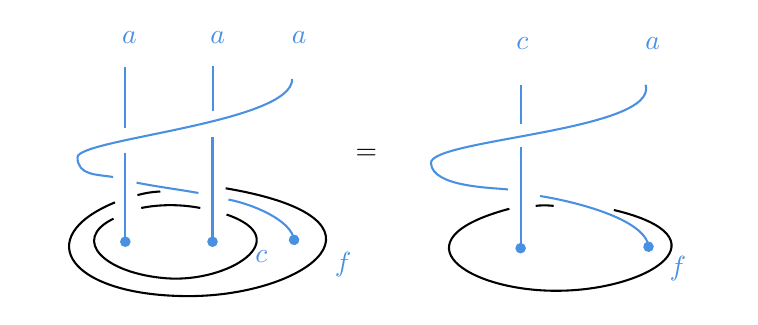
\begin{tikzpicture}[x=0.75pt,y=0.75pt,yscale=-1,xscale=1]
%uncomment if require: \path (0,135); %set diagram left start at 0, and has height of 135

%Curve Lines [id:da4441585115621529] 
\draw    (202.14,82.66) .. controls (160.57,99.82) and (180.38,127.9) .. (237.82,127.83) .. controls (295.26,127.76) and (343.53,90.79) .. (255.44,75.88) ;
%Curve Lines [id:da11147698187779076] 
\draw    (201.42,90.51) .. controls (180.45,100.73) and (197.17,116.99) .. (226.98,119.25) .. controls (256.8,121.51) and (290.23,100.28) .. (255.89,88.53) ;
%Curve Lines [id:da6730479902789113] 
\draw [color={rgb, 255:red, 74; green, 144; blue, 226 }  ,draw opacity=1 ]   (201.23,70.46) .. controls (193.55,69.11) and (184.18,69.9) .. (184.07,60.97) .. controls (183.95,52.05) and (287.72,44.42) .. (287.5,23.23) ;
%Curve Lines [id:da35806285377344316] 
\draw    (214.78,85.37) .. controls (223.82,83.56) and (233.76,83.56) .. (243.24,85.37) ;
%Curve Lines [id:da14528236670523187] 
\draw [color={rgb, 255:red, 74; green, 144; blue, 226 }  ,draw opacity=1 ]   (212.53,73.17) .. controls (224.27,75.43) and (229.24,75.88) .. (242.34,78.14) ;
%Curve Lines [id:da24888935739762763] 
\draw [color={rgb, 255:red, 74; green, 144; blue, 226 }  ,draw opacity=1 ]   (256.8,81.3) .. controls (268.54,83.56) and (287.06,91.24) .. (288.42,100.73) ;
\draw [shift={(288.42,100.73)}, rotate = 81.87] [color={rgb, 255:red, 74; green, 144; blue, 226 }  ,draw opacity=1 ][fill={rgb, 255:red, 74; green, 144; blue, 226 }  ,fill opacity=1 ][line width=0.75]      (0, 0) circle [x radius= 2.01, y radius= 2.01]   ;
%Straight Lines [id:da9560024655558101] 
\draw [color={rgb, 255:red, 74; green, 144; blue, 226 }  ,draw opacity=1 ]   (207.11,58.72) -- (207.11,101.63) ;
\draw [shift={(207.11,101.63)}, rotate = 90] [color={rgb, 255:red, 74; green, 144; blue, 226 }  ,draw opacity=1 ][fill={rgb, 255:red, 74; green, 144; blue, 226 }  ,fill opacity=1 ][line width=0.75]      (0, 0) circle [x radius= 2.01, y radius= 2.01]   ;
%Straight Lines [id:da34660405837493435] 
\draw [color={rgb, 255:red, 74; green, 144; blue, 226 }  ,draw opacity=1 ]   (249.12,51.04) -- (249.12,101.63) ;
\draw [shift={(249.12,101.63)}, rotate = 90] [color={rgb, 255:red, 74; green, 144; blue, 226 }  ,draw opacity=1 ][fill={rgb, 255:red, 74; green, 144; blue, 226 }  ,fill opacity=1 ][line width=0.75]      (0, 0) circle [x radius= 2.01, y radius= 2.01]   ;
%Straight Lines [id:da5382355627625701] 
\draw [color={rgb, 255:red, 74; green, 144; blue, 226 }  ,draw opacity=1 ]   (249.57,17.15) -- (249.57,38.84) ;
%Straight Lines [id:da5288907690406812] 
\draw [color={rgb, 255:red, 74; green, 144; blue, 226 }  ,draw opacity=1 ]   (207.11,17.61) -- (207.11,46.97) ;
%Curve Lines [id:da0812366131709128] 
\draw    (212.96,79.17) .. controls (216.34,78.26) and (219.17,77.7) .. (223.95,77.43) ;

%Curve Lines [id:da744896129398976] 
\draw    (392.13,85.76) .. controls (335.13,100.95) and (371.99,125.89) .. (416.39,125.25) .. controls (460.8,124.61) and (497.83,99.5) .. (442.47,86.33) ;
%Curve Lines [id:da5148656466556178] 
\draw [color={rgb, 255:red, 74; green, 144; blue, 226 }  ,draw opacity=1 ]   (391.55,76.46) .. controls (383.87,75.56) and (354.9,75.32) .. (354.37,63.74) .. controls (353.85,52.16) and (464.15,48.38) .. (457.81,26) ;
%Curve Lines [id:da9281728048283235] 
\draw [color={rgb, 255:red, 74; green, 144; blue, 226 }  ,draw opacity=1 ]   (406.91,79.62) .. controls (421.81,81.88) and (457.95,90.46) .. (459.18,104.04) ;
\draw [shift={(459.18,104.04)}, rotate = 84.84] [color={rgb, 255:red, 74; green, 144; blue, 226 }  ,draw opacity=1 ][fill={rgb, 255:red, 74; green, 144; blue, 226 }  ,fill opacity=1 ][line width=0.75]      (0, 0) circle [x radius= 2.01, y radius= 2.01]   ;
%Curve Lines [id:da1937405317044787] 
\draw    (404.83,84.36) .. controls (406.94,84.09) and (409.76,83.98) .. (413.5,84.36) ;
%Straight Lines [id:da7641241697593497] 
\draw [color={rgb, 255:red, 74; green, 144; blue, 226 }  ,draw opacity=1 ]   (397.56,55.96) -- (397.56,104.75) ;
\draw [shift={(397.56,104.75)}, rotate = 90] [color={rgb, 255:red, 74; green, 144; blue, 226 }  ,draw opacity=1 ][fill={rgb, 255:red, 74; green, 144; blue, 226 }  ,fill opacity=1 ][line width=0.75]      (0, 0) circle [x radius= 2.01, y radius= 2.01]   ;
%Straight Lines [id:da7123297771287953] 
\draw [color={rgb, 255:red, 74; green, 144; blue, 226 }  ,draw opacity=1 ]   (397.56,26.14) -- (397.56,45.11) ;



% Text Node
\draw (204.08,-1) node [anchor=north west][inner sep=0.75pt]  [color={rgb, 255:red, 74; green, 144; blue, 226 }  ,opacity=1 ]  {$a$};
% Text Node
\draw (246.54,-1) node [anchor=north west][inner sep=0.75pt]  [color={rgb, 255:red, 74; green, 144; blue, 226 }  ,opacity=1 ]  {$a$};
% Text Node
\draw (285.84,-1) node [anchor=north west][inner sep=0.75pt]  [color={rgb, 255:red, 74; green, 144; blue, 226 }  ,opacity=1 ]  {$a$};
% Text Node
\draw (268.22,104.29) node [anchor=north west][inner sep=0.75pt]  [color={rgb, 255:red, 74; green, 144; blue, 226 }  ,opacity=1 ]  {$c$};
% Text Node
\draw (306.62,105.2) node [anchor=north west][inner sep=0.75pt]  [color={rgb, 255:red, 74; green, 144; blue, 226 }  ,opacity=1 ]  {$f$};
% Text Node
\draw (394.08,1.57) node [anchor=north west][inner sep=0.75pt]  [color={rgb, 255:red, 74; green, 144; blue, 226 }  ,opacity=1 ]  {$c$};
% Text Node
\draw (456.15,1.57) node [anchor=north west][inner sep=0.75pt]  [color={rgb, 255:red, 74; green, 144; blue, 226 }  ,opacity=1 ]  {$a$};
% Text Node
\draw (467.9,107.06) node [anchor=north west][inner sep=0.75pt]  [color={rgb, 255:red, 74; green, 144; blue, 226 }  ,opacity=1 ]  {$f$};
% Text Node
\draw (316.61,55.42) node [anchor=north west][inner sep=0.75pt]    {$=$};
\end{tikzpicture}
\caption{The locality constraint of $a,a,a$.}
\label{fig:localityAAA}
\end{figure}

\begin{figure}[h!]
\centering
\tikzset{every picture/.style={line width=0.75pt}} %set default line width to 0.75pt        

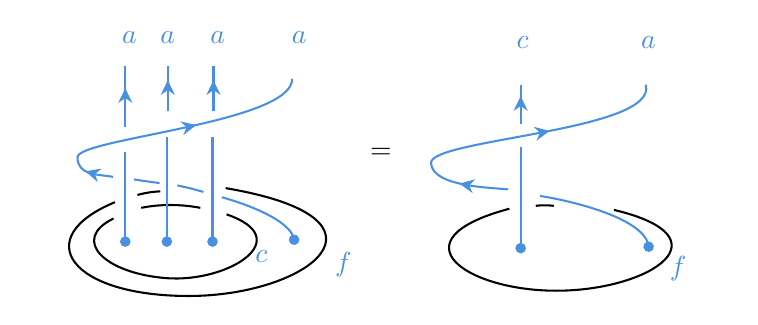
\begin{tikzpicture}[x=0.75pt,y=0.75pt,yscale=-1,xscale=1]
%uncomment if require: \path (0,137); %set diagram left start at 0, and has height of 137

%Curve Lines [id:da48005012890803767] 
\draw [color={rgb, 255:red, 74; green, 144; blue, 226 }  ,draw opacity=1 ]   (406.92,84.56) .. controls (421.83,86.82) and (457.98,95.4) .. (459.2,108.99) ;
\draw [shift={(459.2,108.99)}, rotate = 84.84] [color={rgb, 255:red, 74; green, 144; blue, 226 }  ,draw opacity=1 ][fill={rgb, 255:red, 74; green, 144; blue, 226 }  ,fill opacity=1 ][line width=0.75]      (0, 0) circle [x radius= 2.01, y radius= 2.01]   ;
%Curve Lines [id:da48455883811391565] 
\draw    (392.14,90.7) .. controls (335.13,105.89) and (372,130.83) .. (416.41,130.19) .. controls (460.82,129.55) and (497.86,104.44) .. (442.49,91.26) ;
%Curve Lines [id:da8722293198278814] 
\draw [color={rgb, 255:red, 74; green, 144; blue, 226 }  ,draw opacity=1 ]   (391.56,81.4) .. controls (383.88,80.49) and (354.9,80.25) .. (354.38,68.67) .. controls (353.86,57.09) and (464.17,53.31) .. (457.83,30.92) ;
\draw [shift={(368.08,78.57)}, rotate = 10.58] [fill={rgb, 255:red, 74; green, 144; blue, 226 }  ,fill opacity=1 ][line width=0.08]  [draw opacity=0] (7.14,-3.43) -- (0,0) -- (7.14,3.43) -- (4.74,0) -- cycle    ;
\draw [shift={(411.49,53.22)}, rotate = 168.97] [fill={rgb, 255:red, 74; green, 144; blue, 226 }  ,fill opacity=1 ][line width=0.08]  [draw opacity=0] (7.14,-3.43) -- (0,0) -- (7.14,3.43) -- (4.74,0) -- cycle    ;
%Curve Lines [id:da6534979362287627] 
\draw    (404.84,89.3) .. controls (406.95,89.03) and (409.78,88.91) .. (413.52,89.3) ;
%Straight Lines [id:da6201900126274491] 
\draw [color={rgb, 255:red, 74; green, 144; blue, 226 }  ,draw opacity=1 ]   (397.57,60.89) -- (397.57,109.69) ;
\draw [shift={(397.57,109.69)}, rotate = 90] [color={rgb, 255:red, 74; green, 144; blue, 226 }  ,draw opacity=1 ][fill={rgb, 255:red, 74; green, 144; blue, 226 }  ,fill opacity=1 ][line width=0.75]      (0, 0) circle [x radius= 2.01, y radius= 2.01]   ;
%Straight Lines [id:da3482404205300744] 
\draw [color={rgb, 255:red, 74; green, 144; blue, 226 }  ,draw opacity=1 ]   (397.57,31.07) -- (397.57,50.05) ;
\draw [shift={(397.57,36.46)}, rotate = 90] [fill={rgb, 255:red, 74; green, 144; blue, 226 }  ,fill opacity=1 ][line width=0.08]  [draw opacity=0] (7.14,-3.43) -- (0,0) -- (7.14,3.43) -- (4.74,0) -- cycle    ;

%Curve Lines [id:da08063743561300551] 
\draw    (202.11,87.55) .. controls (160.55,104.72) and (180.36,132.81) .. (237.81,132.74) .. controls (295.26,132.67) and (343.54,95.69) .. (255.43,80.78) ;
%Curve Lines [id:da5619779829028049] 
\draw    (201.4,95.41) .. controls (180.43,105.63) and (197.14,121.89) .. (226.96,124.15) .. controls (256.79,126.41) and (290.22,105.18) .. (255.88,93.43) ;
%Curve Lines [id:da048092793307539905] 
\draw [color={rgb, 255:red, 74; green, 144; blue, 226 }  ,draw opacity=1 ]   (201.21,75.35) .. controls (193.53,74) and (184.15,74.79) .. (184.04,65.87) .. controls (183.93,56.94) and (287.71,49.31) .. (287.49,28.12) ;
\draw [shift={(187.92,72.67)}, rotate = 16.03] [fill={rgb, 255:red, 74; green, 144; blue, 226 }  ,fill opacity=1 ][line width=0.08]  [draw opacity=0] (7.14,-3.43) -- (0,0) -- (7.14,3.43) -- (4.74,0) -- cycle    ;
\draw [shift={(241.24,50.38)}, rotate = 167.43] [fill={rgb, 255:red, 74; green, 144; blue, 226 }  ,fill opacity=1 ][line width=0.08]  [draw opacity=0] (7.14,-3.43) -- (0,0) -- (7.14,3.43) -- (4.74,0) -- cycle    ;
%Curve Lines [id:da17248471812798782] 
\draw    (214.77,90.27) .. controls (223.8,88.46) and (233.74,88.46) .. (243.23,90.27) ;
%Curve Lines [id:da7603279216217766] 
\draw [color={rgb, 255:red, 74; green, 144; blue, 226 }  ,draw opacity=1 ]   (211.31,76.61) .. controls (215.31,77.18) and (218.74,77.75) .. (223.6,78.32) ;
%Curve Lines [id:da8804125859785752] 
\draw [color={rgb, 255:red, 74; green, 144; blue, 226 }  ,draw opacity=1 ]   (253.6,85.18) .. controls (264.17,88.04) and (287.06,96.14) .. (288.41,105.63) ;
\draw [shift={(288.41,105.63)}, rotate = 81.87] [color={rgb, 255:red, 74; green, 144; blue, 226 }  ,draw opacity=1 ][fill={rgb, 255:red, 74; green, 144; blue, 226 }  ,fill opacity=1 ][line width=0.75]      (0, 0) circle [x radius= 2.01, y radius= 2.01]   ;
%Straight Lines [id:da7272638799250273] 
\draw [color={rgb, 255:red, 74; green, 144; blue, 226 }  ,draw opacity=1 ]   (207.08,63.61) -- (207.08,106.53) ;
\draw [shift={(207.08,106.53)}, rotate = 90] [color={rgb, 255:red, 74; green, 144; blue, 226 }  ,draw opacity=1 ][fill={rgb, 255:red, 74; green, 144; blue, 226 }  ,fill opacity=1 ][line width=0.75]      (0, 0) circle [x radius= 2.01, y radius= 2.01]   ;
%Straight Lines [id:da7356806877559408] 
\draw [color={rgb, 255:red, 74; green, 144; blue, 226 }  ,draw opacity=1 ]   (249.1,55.93) -- (249.1,106.53) ;
\draw [shift={(249.1,106.53)}, rotate = 90] [color={rgb, 255:red, 74; green, 144; blue, 226 }  ,draw opacity=1 ][fill={rgb, 255:red, 74; green, 144; blue, 226 }  ,fill opacity=1 ][line width=0.75]      (0, 0) circle [x radius= 2.01, y radius= 2.01]   ;
%Straight Lines [id:da10030509523856646] 
\draw [color={rgb, 255:red, 74; green, 144; blue, 226 }  ,draw opacity=1 ]   (249.56,22.04) -- (249.56,43.73) ;
\draw [shift={(249.56,28.78)}, rotate = 90] [fill={rgb, 255:red, 74; green, 144; blue, 226 }  ,fill opacity=1 ][line width=0.08]  [draw opacity=0] (7.14,-3.43) -- (0,0) -- (7.14,3.43) -- (4.74,0) -- cycle    ;
%Straight Lines [id:da5226385743371742] 
\draw [color={rgb, 255:red, 74; green, 144; blue, 226 }  ,draw opacity=1 ]   (207.08,22.04) -- (207.08,51.41) ;
\draw [shift={(207.08,32.62)}, rotate = 90] [fill={rgb, 255:red, 74; green, 144; blue, 226 }  ,fill opacity=1 ][line width=0.08]  [draw opacity=0] (7.14,-3.43) -- (0,0) -- (7.14,3.43) -- (4.74,0) -- cycle    ;
%Curve Lines [id:da07495684145792891] 
\draw    (212.94,84.06) .. controls (216.32,83.16) and (219.15,82.6) .. (223.93,82.33) ;
%Straight Lines [id:da5752086666094567] 
\draw [color={rgb, 255:red, 74; green, 144; blue, 226 }  ,draw opacity=1 ]   (227.1,55.93) -- (227.1,106.53) ;
\draw [shift={(227.1,106.53)}, rotate = 90] [color={rgb, 255:red, 74; green, 144; blue, 226 }  ,draw opacity=1 ][fill={rgb, 255:red, 74; green, 144; blue, 226 }  ,fill opacity=1 ][line width=0.75]      (0, 0) circle [x radius= 2.01, y radius= 2.01]   ;
%Straight Lines [id:da5198457266167438] 
\draw [color={rgb, 255:red, 74; green, 144; blue, 226 }  ,draw opacity=1 ]   (227.56,22.04) -- (227.56,43.73) ;
\draw [shift={(227.56,28.78)}, rotate = 90] [fill={rgb, 255:red, 74; green, 144; blue, 226 }  ,fill opacity=1 ][line width=0.08]  [draw opacity=0] (7.14,-3.43) -- (0,0) -- (7.14,3.43) -- (4.74,0) -- cycle    ;
%Curve Lines [id:da609532659113271] 
\draw [color={rgb, 255:red, 74; green, 144; blue, 226 }  ,draw opacity=1 ]   (232.17,79.47) .. controls (236.17,80.32) and (238.74,80.9) .. (244.74,82.61) ;



% Text Node
\draw (323.58,60.35) node [anchor=north west][inner sep=0.75pt]    {$=$};
% Text Node
\draw (222.53,3.97) node [anchor=north west][inner sep=0.75pt]  [color={rgb, 255:red, 74; green, 144; blue, 226 }  ,opacity=1 ]  {$a$};
% Text Node
\draw (306.62,110.1) node [anchor=north west][inner sep=0.75pt]  [color={rgb, 255:red, 74; green, 144; blue, 226 }  ,opacity=1 ]  {$f$};
% Text Node
\draw (268.21,109.19) node [anchor=north west][inner sep=0.75pt]  [color={rgb, 255:red, 74; green, 144; blue, 226 }  ,opacity=1 ]  {$c$};
% Text Node
\draw (285.84,3.97) node [anchor=north west][inner sep=0.75pt]  [color={rgb, 255:red, 74; green, 144; blue, 226 }  ,opacity=1 ]  {$a$};
% Text Node
\draw (246.53,3.97) node [anchor=north west][inner sep=0.75pt]  [color={rgb, 255:red, 74; green, 144; blue, 226 }  ,opacity=1 ]  {$a$};
% Text Node
\draw (204.05,3.97) node [anchor=north west][inner sep=0.75pt]  [color={rgb, 255:red, 74; green, 144; blue, 226 }  ,opacity=1 ]  {$a$};
% Text Node
\draw (467.92,112) node [anchor=north west][inner sep=0.75pt]  [color={rgb, 255:red, 74; green, 144; blue, 226 }  ,opacity=1 ]  {$f$};
% Text Node
\draw (454.17,6.5) node [anchor=north west][inner sep=0.75pt]  [color={rgb, 255:red, 74; green, 144; blue, 226 }  ,opacity=1 ]  {$a$};
% Text Node
\draw (394.09,6.5) node [anchor=north west][inner sep=0.75pt]  [color={rgb, 255:red, 74; green, 144; blue, 226 }  ,opacity=1 ]  {$c$};
\end{tikzpicture}
\caption{The locality constraint of $a,a,a,a$.}
\label{fig:localityAAAA}
\end{figure}

\noindent (Hard) Consider the braid shown on the left of Fig.\ref{fig:localityAAAA}. The braid can be written as $\hat{b}_{4} =\hat{\sigma }_{3}\hat{\sigma }_{2}\hat{\sigma }_{1}^{2}\hat{\sigma }_{2}\hat{\sigma }_{3}$.

\begin{enumerate}
\setcounter{enumi}{2}
\item Consider Ising anyons where $a=\sigma $, Use the $F$ and $R$-matrices to calculate $\hat{\sigma }_{3}$ (See exercise 10.3.a). Since the fusion of three $\sigma $ anyons always gives $c=\sigma $, calculate $\hat{b}_{4}$, show this is a phase times the identity matrix, and show that the phase matches the phase of taking a single $\sigma $ all the way around another $\sigma $.
\item Consider Fibonacci anyons with $a=\tau $, Use the $F$ and $R$-matrices to calculate $\hat{\sigma }_{3}$. (See exercise 10.3.b). Check that $\hat{b}_{4}$ is a diagonal matrix of phases. Check the phases match the two possible phases accumulated by wrapping a single $\tau $ all the way around a single particle $c$ which can be $I$ or $\tau $.
\end{enumerate}

\paragraph{Answer}
(a) For Fibonacci anyons, these two braiding operators are given by
\begin{equation*}
\hat{\sigma }_{1} =\begin{pmatrix}
\mathrm{e}^{3\pi \mathrm{i} /5} &  & \\
 & \mathrm{e}^{-4\pi \mathrm{i} /5} & \\
 &  & \mathrm{e}^{3\pi \mathrm{i} /5}
\end{pmatrix} ,\quad \hat{\sigma }_{2} =\begin{pmatrix}
\mathrm{e}^{3\pi \mathrm{i} /5} & 0 & 0\\
0 & \phi ^{-1}\mathrm{e}^{4\pi \mathrm{i} /5} & \phi ^{-1/2}\mathrm{e}^{-3\pi \mathrm{i} /5}\\
0 & \phi ^{-1/2}\mathrm{e}^{-3\pi \mathrm{i} /5} & -\phi ^{-1}
\end{pmatrix} .
\end{equation*}
Direct calculation gives
\begin{equation*}
\hat{b}_{3} =\hat{\sigma }_{2}\hat{\sigma }_{1}^{2}\hat{\sigma }_{2} =\begin{pmatrix}
\mathrm{e}^{2\pi \mathrm{i} /5} &  & \\
 & 1 & \\
 &  & \mathrm{e}^{-4\pi \mathrm{i} /5}
\end{pmatrix} ,
\end{equation*}
which is a diagonal matrix of complex phases. Note that in this process, $c$ only have two possibilities, i.e. $I,\tau $, and the final result $f$ corresponds $I,\tau $, we know that
\begin{equation*}
\begin{aligned}
\hat{b}_{3} |N\rangle  & =(R_{I}^{c\tau } )^{2} =(R_{I}^{\tau \tau } )^{2} =\mathrm{e}^{-8\pi \mathrm{i} /5} =\mathrm{e}^{2\pi \mathrm{i} /5} ,\\
\hat{b}_{3} |0\rangle  & =(R_{\tau }^{c\tau } )^{2} =(R_{\tau }^{I\tau } )^{2} =1,\\
\hat{b}_{3} |1\rangle  & =(R_{\tau }^{c\tau } )^{2} =(R_{\tau }^{\tau \tau } )^{2} =\mathrm{e}^{6\pi \mathrm{i} /5} =\mathrm{e}^{-4\pi \mathrm{i} /5} .
\end{aligned}
\end{equation*}
So these phases are the same as the phase that would be accumulated for taking a single $\tau $ particle around the particle $c$.



(b) For Ising anyons, the two braiding operators are given by
\begin{equation*}
\hat{\sigma }_{1} =\mathrm{e}^{-\mathrm{i} \pi /8}\begin{pmatrix}
1 & 0\\
0 & \mathrm{i}
\end{pmatrix} ,\quad \hat{\sigma }_{2} =\frac{\mathrm{e}^{\mathrm{i} \pi /8}}{\sqrt{2}}\begin{pmatrix}
1 & -\mathrm{i}\\
-\mathrm{i} & 1
\end{pmatrix} .
\end{equation*}
Direct calculation gives
\begin{equation*}
\hat{b}_{3} =\hat{\sigma }_{2}\hat{\sigma }_{1}^{2}\hat{\sigma }_{2} =\begin{pmatrix}
1 & \\
 & -1
\end{pmatrix} .
\end{equation*}
Which indicates that actually $(R_{\sigma }^{\psi \sigma } )^{2} =\hat{b}_{3} |1 \rangle =-1$. 



(c) For Ising anyons, we have already calculate that
\begin{equation*}
\hat{\sigma }_{3} =\begin{pmatrix}
\mathrm{e}^{3\pi \mathrm{i} /8} & 0\\
0 & \mathrm{e}^{-\mathrm{i} \pi /8}
\end{pmatrix} .
\end{equation*}
Therefore, we have
\begin{equation*}
\hat{b}_{4} =\hat{\sigma }_{3}\hat{\sigma }_{2}\hat{\sigma }_{1}^{2}\hat{\sigma }_{2}\hat{\sigma }_{3} =\mathrm{e}^{3\pi \mathrm{i} /4}\begin{pmatrix}
1 & \\
 & 1
\end{pmatrix} ,
\end{equation*}
which is a phase times the identity matrix. We know that four Ising anyons can only fusion to $\psi $, so the phase must equals to $(R_{\psi }^{\sigma \sigma } )^{2} =(\mathrm{e}^{3\pi \mathrm{i} /8} )^{2} =\mathrm{e}^{3\pi \mathrm{i} /4}$, which is exactly the case. 



(d) According to our calculation result \eqref{eq:FibBraiding3}:
\begin{equation*}
\hat{b}_{4} =\hat{\sigma }_{3}\hat{\sigma }_{2}\hat{\sigma }_{1}^{2}\hat{\sigma }_{2}\hat{\sigma }_{3} =\operatorname{diag} (\mathrm{e}^{2\pi \mathrm{i} /5} ,\mathrm{e}^{2\pi \mathrm{i} /5} ,\mathrm{e}^{-4\pi \mathrm{i} /5} ,\mathrm{e}^{-4\pi \mathrm{i} /5} ,1).
\end{equation*}
This is actually the case:
\begin{equation*}
\begin{aligned}
\hat{b}_{4} |0;I\rangle =\hat{b}_{4} |1;I \rangle  & =(R_{I}^{\tau \tau } )^{2} =\mathrm{e}^{2\pi \mathrm{i} /5} ,\\
\hat{b}_{4} |-1;I\rangle =\hat{b}_{4} |0;I \rangle  & =(R_{\tau }^{\tau \tau } )^{2} =\mathrm{e}^{-4\pi \mathrm{i} /5} ,\\
\hat{b}_{4} |1;I \rangle  & =(R_{\tau }^{\tau I} )^{2} =1.
\end{aligned}
\end{equation*}


\section{Enforcing the locality constraint}
The locality constraint shown in Fig.\ref{fig:localityAAA} turns out to be extremely powerful. In this exercise we will use this constraint to (almost) derive the possible values for the $R$-matrix for Fibonacci anyons given the known $F$-matrix.

Consider an anyon theory with Fibonacci fusion rules and Fibonacci $F$ matrix as in Eq. 9.2.
\begin{enumerate}
\item (Easy) Confirm the locality constraint shown in Fig.\ref{fig:localityAAA} (see also Fig. \ref{fig:localityAAAA}) given the values of $R$ given in Eq. 10.2. Make sure to confirm the equality for all three cases $f=I,c=\tau $ and $f=\tau ,c=I$ and $f=\tau ,c=\tau $. 

Note that on the left of Fig. $10.16$ is the braiding operation $\hat{O} =\hat{\sigma }_{2}\hat{\sigma }_{1}\hat{\sigma }_{1}\hat{\sigma }_{2}$. whereas the operation on the right is $\sigma ^{2}$.
\item Show that the locality constraint of Fig.\ref{fig:localityAAA} would also be satisfied by\begin{equation*}
R_{I}^{\tau \tau }\rightarrow -R_{I}^{\tau \tau } \ \ R_{\tau }^{\tau \tau }\rightarrow -R_{\tau }^{\tau \tau }
\end{equation*}It will turn out (See $^{***}$ below) that this additional solution is spurious, as there are other consistency conditions it does not satisfy.
\item In addition to right and left handed Fibonacci anyons and the two additional spurious solutions provided by Eq. 10.14, there are four additional possible sets of $R$-matrices that are consistent with the $F$-matrices of the Fibonacci theory given the locality constraint of Fig. 10.16. These additional solutions are all fairly trivial. Can you guess any of them?

If we cannot guess the additional possible $R$-matrices, we can derive them explicitly (and show that no others exist). Let us suppose that we do not know the values of the $R$-matrix elements $R_{I}^{\tau \tau }$ and $R_{\tau }^{\tau \tau }$.
\item For the case of $f=I$ and $c=\tau $ show that Fig. $10.16$ implies\begin{equation*}
[R_{\tau }^{\tau \tau } ]^{4} =[R_{I}^{\tau \tau } ]^{2}
\end{equation*}
\item (Harder) For the case of $f=\tau $ we have a two-dimensional Hilbert space spanned by the two values of $c=I$ or $c=\tau $. Any linear operator on this Hilbert space should be a 2 by 2 matrix. Thus the locality constraint Eq. $10.16$ is actually an equality of 2 by 2 matrices. Derive this equality.
\item Use this result, in combination with Eq. $10.15$ to find all possible $R$ matrices that satisfy the locality constraint. You should find a total of eight solutions. Six of these are spurious as we will see in section 13.3.

The calculation you have just done is equivalent to enforcing the so-called hexagon condition which we will discuss in section $13.3$ below.
\end{enumerate}

\paragraph{Answer}
(a) As we have checked before:
\begin{equation*}
\begin{aligned}
\hat{b}_{3} |N\rangle  & =(R_{f}^{c\tau } )^{2} =(R_{I}^{\tau \tau } )^{2} =\mathrm{e}^{-8\pi \mathrm{i} /5} =\mathrm{e}^{2\pi \mathrm{i} /5} ,\\
\hat{b}_{3} |0\rangle  & =(R_{f}^{c\tau } )^{2} =(R_{\tau }^{I\tau } )^{2} =1,\\
\hat{b}_{3} |1\rangle  & =(R_{f}^{c\tau } )^{2} =(R_{\tau }^{\tau \tau } )^{2} =\mathrm{e}^{6\pi \mathrm{i} /5} =\mathrm{e}^{-4\pi \mathrm{i} /5} ,
\end{aligned}
\end{equation*}
which gives
\begin{equation*}
\hat{b}_{3} =\begin{pmatrix}
\mathrm{e}^{2\pi \mathrm{i} /5} &  & \\
 & 1 & \\
 &  & \mathrm{e}^{-4\pi \mathrm{i} /5}
\end{pmatrix} .
\end{equation*}


(b) From the Fig.\ref{fig:localityAAA}, we can see that $\tau $ braids around $f$ twice, which means the result will always be $(R_{f}^{c\tau } )^{2}$. So it is invariant under the transformation $R_{f}^{c\tau }\rightarrow -R_{f}^{c\tau }$. 



(c) A fairly trivial guess is that
\begin{equation*}
R_{\tau }^{I\tau } =R_{\tau }^{\tau I} =1.
\end{equation*}
This can be checked by the hexagon identity using $F_{\tau }^{\tau \tau I} =F_{I}^{\tau \tau \tau } =1$. 



(d) We have already figure out that the right part of Fig.\ref{fig:localityAAA} is:
\begin{equation*}
\hat{b}_{3} |N \rangle =(R_{I}^{\tau \tau } )^{2} .
\end{equation*}
While the left part of Fig.\ref{fig:localityAAA} is
\begin{equation*}
\begin{aligned}
\hat{\sigma }_{2}\hat{\sigma }_{1}\hat{\sigma }_{1}\hat{\sigma }_{2} |N \rangle  & =\hat{\sigma }_{2}\hat{\sigma }_{1}\hat{\sigma }_{1}\hat{\sigma }_{2} F_{I}^{\tau \tau \tau }\tikzset{every picture/.style={line width=0.75pt}} %set default line width to 0.75pt        
\begin{tikzpicture}[x=0.75pt,y=0.75pt,yscale=-1,xscale=1, baseline=(XXXX.south) ]
\path (0,70);\path (94.97024536132812,0);\draw    ($(current bounding box.center)+(0,0.3em)$) node [anchor=south] (XXXX) {};
%Straight Lines [id:da7556404348647627] 
\draw [color={rgb, 255:red, 74; green, 144; blue, 226 }  ,draw opacity=1 ]   (1.97,6.96) -- (41.97,46.96) ;
%Straight Lines [id:da8420662452631105] 
\draw [color={rgb, 255:red, 74; green, 144; blue, 226 }  ,draw opacity=1 ]   (61.97,26.96) -- (41.97,6.96) ;
%Straight Lines [id:da47708456812367284] 
\draw [color={rgb, 255:red, 74; green, 144; blue, 226 }  ,draw opacity=1 ]   (41.97,46.96) -- (81.97,6.96) ;
%Straight Lines [id:da3162472235386862] 
\draw [color={rgb, 255:red, 74; green, 144; blue, 226 }  ,draw opacity=1 ] [dash pattern={on 0.84pt off 2.51pt}]  (41.97,46.96) -- (61.97,66.96) ;
% Text Node
\draw (9.97,-0.54) node [anchor=north west][inner sep=0.75pt]    {$\tau $};
% Text Node
\draw (46.97,-0.54) node [anchor=north west][inner sep=0.75pt]    {$\tau $};
% Text Node
\draw (82.97,-0.54) node [anchor=north west][inner sep=0.75pt]    {$\tau $};
% Text Node
\draw (54.97,28.46) node [anchor=north west][inner sep=0.75pt]    {$\tau $};
% Text Node
\draw (38.97,53.46) node [anchor=north west][inner sep=0.75pt]    {$I$};
\end{tikzpicture}
\\
 & =\hat{\sigma }_{2}\hat{\sigma }_{1}\hat{\sigma }_{1} R_{\tau }^{\tau \tau }\tikzset{every picture/.style={line width=0.75pt}} %set default line width to 0.75pt        
\begin{tikzpicture}[x=0.75pt,y=0.75pt,yscale=-1,xscale=1, baseline=(XXXX.south) ]
\path (0,70);\path (94.97024536132812,0);\draw    ($(current bounding box.center)+(0,0.3em)$) node [anchor=south] (XXXX) {};
%Straight Lines [id:da20932905132062474] 
\draw [color={rgb, 255:red, 74; green, 144; blue, 226 }  ,draw opacity=1 ]   (1.97,6.96) -- (41.97,46.96) ;
%Straight Lines [id:da6844706933147437] 
\draw [color={rgb, 255:red, 74; green, 144; blue, 226 }  ,draw opacity=1 ]   (61.97,26.96) -- (41.97,6.96) ;
%Straight Lines [id:da4159700799839392] 
\draw [color={rgb, 255:red, 74; green, 144; blue, 226 }  ,draw opacity=1 ]   (41.97,46.96) -- (81.97,6.96) ;
%Straight Lines [id:da7259501798903829] 
\draw [color={rgb, 255:red, 74; green, 144; blue, 226 }  ,draw opacity=1 ] [dash pattern={on 0.84pt off 2.51pt}]  (41.97,46.96) -- (61.97,66.96) ;
% Text Node
\draw (9.97,-0.54) node [anchor=north west][inner sep=0.75pt]    {$\tau $};
% Text Node
\draw (46.97,-0.54) node [anchor=north west][inner sep=0.75pt]    {$\tau $};
% Text Node
\draw (82.97,-0.54) node [anchor=north west][inner sep=0.75pt]    {$\tau $};
% Text Node
\draw (54.97,28.46) node [anchor=north west][inner sep=0.75pt]    {$\tau $};
% Text Node
\draw (38.97,53.46) node [anchor=north west][inner sep=0.75pt]    {$I$};
\end{tikzpicture}
\\
 & =R_{\tau }^{\tau \tau }\hat{\sigma }_{2}\hat{\sigma }_{1}\hat{\sigma }_{1} |N \rangle \\
 & =(R_{\tau }^{\tau \tau } )^{3}\hat{\sigma }_{2} |N \rangle =(R_{\tau }^{\tau \tau } )^{4} .
\end{aligned}
\end{equation*}
So without knowing the exact value of $R_{\tau }^{\tau \tau }$ and $R_{I}^{\tau \tau }$, we can give the relation $(R_{\tau }^{\tau \tau } )^{4} =(R_{I}^{\tau \tau } )^{2}$ directly from the locality constraints. 


(e) Without knowing the exact value of $R_{I}^{\tau \tau } ,R_{\tau }^{\tau \tau }$, we can just write
\begin{equation*}
\hat{\sigma }_{1} =\begin{pmatrix}
R_{I}^{\tau \tau } & \\
 & R_{\tau }^{\tau \tau }
\end{pmatrix} ,\quad \hat{\sigma }_{2} =\begin{pmatrix}
\phi ^{-2} R_{I}^{\tau \tau } +\phi ^{-1} R_{\tau }^{\tau \tau } & \phi ^{-3/2} (R_{I}^{\tau \tau } -R_{\tau }^{\tau \tau } )\\
\phi ^{-3/2} (R_{I}^{\tau \tau } -R_{\tau }^{\tau \tau } ) & \phi ^{-1} R_{I}^{\tau \tau } +\phi ^{-2} R_{\tau }^{\tau \tau }
\end{pmatrix} .
\end{equation*}
We further know that with $f=\tau ,c=I,\tau $
\begin{equation*}
\hat{b}_{3} =\begin{pmatrix}
(R_{I}^{\tau \tau } )^{2} & \\
 & (R_{\tau }^{\tau \tau } )^{2}
\end{pmatrix}\stackrel{!}{=}\hat{\sigma }_{2}\hat{\sigma }_{1}^{2}\hat{\sigma }_{2} .
\end{equation*}
This gives three equations:
\begin{equation*}
\begin{aligned}
(R_{I}^{\tau \tau } )^{2} & =\frac{(R_{I}^{\tau \tau } )^{2} (\phi R_{\tau }^{\tau \tau } +R_{I}^{\tau \tau } )^{2} +\phi (R_{\tau }^{\tau \tau } )^{2} (R_{I}^{\tau \tau } -R_{\tau }^{\tau \tau } )^{2}}{\phi ^{4}} ,\\
0 & =\frac{(R_{\tau }^{\tau \tau } -R_{I}^{\tau \tau } )(\phi (R_{I}^{\tau \tau } )^{2} R_{\tau }^{\tau \tau } +\phi R_{I}^{\tau \tau } (R_{\tau }^{\tau \tau } )^{2} +(R_{I}^{\tau \tau } )^{3} +(R_{\tau }^{\tau \tau } )^{3} )}{\phi ^{7/2}} ,\\
(R_{\tau }^{\tau \tau } )^{2} & =\frac{\phi (R_{I}^{\tau \tau } )^{2} (R_{I}^{\tau \tau } -R_{\tau }^{\tau \tau } )^{2} +(R_{\tau }^{\tau \tau } )^{2} (\phi R_{I}^{\tau \tau } +R_{\tau }^{\tau \tau } )^{2}}{\phi ^{4}} .
\end{aligned}
\end{equation*}


(f) The second equation can be reduced to:
\begin{equation*}
(R_{I}^{\tau \tau } -R_{\tau }^{\tau \tau } )(R_{I}^{\tau \tau } +R_{\tau }^{\tau \tau } )((R_{I}^{\tau \tau } )^{2} +\phi ^{-1} R_{I}^{\tau \tau } R_{\tau }^{\tau \tau } +(R_{\tau }^{\tau \tau } )^{2} )=0.
\end{equation*}
We have solutions
\begin{equation*}
\frac{R_{I}^{\tau \tau }}{R_{\tau }^{\tau \tau }} =\pm 1,\mathrm{e}^{\pm 7\pi \mathrm{i} /5} .
\end{equation*}
With $(R_{\tau }^{\tau \tau } )^{4} =(R_{I}^{\tau \tau } )^{2}$, we have eight solutions
\begin{equation*}
(R_{I}^{\tau \tau } ,R_{\tau }^{\tau \tau } )=(\pm 1,\pm 1),(\pm 1,\mp 1),(\mathrm{e}^{\pm \mathrm{i} \pi /5} ,\mathrm{e}^{\mp 2\pi \mathrm{i} /5} ),(\mathrm{e}^{\mp 4\pi \mathrm{i} /5} ,\mathrm{e}^{\pm 3\pi \mathrm{i} /5} ).
\end{equation*}
We can plug these solutions into other two equation to examine these solutions are correct. The last two solutions are physical, which is the left and right handed Fibonacci anyons. 
